%
% Einfache LaTeX-Vorlage f�r Arbeiten am Lehrstuhl Kranzlm�ller / MNM-Team
% - optimiert f�r die Arbeit mit g�ngigen LaTeX-Editoren
% - funktioniert ohne Makefile und Anpassungen der LaTeX-Verzeichnisstruktur
% - verwendet Komaskript f�r ein (nach europ�ischen Gepflogenheiten) sch�neres Layout
% 
% v1, 2007 (Michael Brenner)
% Diese Version: v1.1, 2012 (Michael Brenner)
%


\documentclass[bibliography=totoc,listof=totoc,BCOR=5mm,DIV=12]{scrbook} % Rand f�r Bindung: 5mm / falls Index verwendet, erg�nze "index=totoc" zu den Optionen 
\usepackage{bibgerm}       % deutsche Literaturverzeichnisse
\usepackage[latin1]{inputenc} % Umlaute im Text
\usepackage{graphicx} % Einf�gen von Grafiken  - f�r PDF-Latex: .pdf und .png (.jpg m�glich, sollte aber vermieden werden)
\usepackage{url}           % URL's (z.B. in Literatur) sch�ner formatieren
\usepackage{hyperref} % sorgt f�r f�r Hyperlinks in PDF-Dokumenten
\usepackage{setspace}
\usepackage{here}
\usepackage{amsmath}
\usepackage{color}

\graphicspath{{./Bilder/}}

%
% der Befehl \hyphenation versteht keine Sonderzeichen, also weder �
% noch "a noch \"a. W�rter die derartige Zeichen enthalten m�ssen
% direkt im Text getrennt werden, z.B. W�r\-ter
%
\hyphenation{Ma-nage-ment}
\hyphenation{Ma-nage-ment-agent}
\hyphenation{Ma-nage-ment-agent-en}
\hyphenation{Ma-nage-ment-ar-chi-tek-tur}
\hyphenation{Ma-nage-ment-ar-chi-tek-tu-ren}
\hyphenation{Ma-nage-ment-an-wen-dung}
\hyphenation{Ma-nage-ment-an-wen-dung-en}
\hyphenation{Ma-nage-ment-an-for-der-ung}
\hyphenation{Ma-nage-ment-funk-ti-on}
\hyphenation{Ma-nage-ment-funk-ti-onen}
\hyphenation{Ma-nage-ment-kon-zep-te}
\hyphenation{Ma-nage-ment-res-source}
\hyphenation{Ma-nage-ment-in-for-ma-ti-on}
\hyphenation{Ma-nage-ment-res-sour-cen}
\hyphenation{ma-nage-ment-re-le-vante}
\hyphenation{ma-nage-ment-sy-stem}
\hyphenation{ma-nage-ment-sy-steme}
\hyphenation{Ma-nage-ment-in-stru-men-tie-rung}
\hyphenation{Ma-nage-ment-platt-form}
\hyphenation{Sys-te-men}
\hyphenation{Sys-tem-um-ge-bun-gen}
\hyphenation{Sys-tem-ma-nage-ment}
\hyphenation{DHCP}
\hyphenation{Ma-nage-ment-diszi-plinen}
\hyphenation{System-management-architekturen}
\hyphenation{Verwendungs-nachweise}
\hyphenation{Video-einricht-ungen}
\hyphenation{Res-source}
\hyphenation{Res-sourcen}
\hyphenation{Grund-anwendung}
\hyphenation{Grund-anwendungen}
\hyphenation{Basis-anwendung}
\hyphenation{Core}
\hyphenation{Kom-mu-ni-ka-ti-on}
\hyphenation{De-sign-ent-schei-dung}
\hyphenation{Sprung-ad-res-sen}
\hyphenation{Klas-si-fi-ka-ti-on}
\hyphenation{Schreib-recht}
\hyphenation{Be-nut-zer-zer-ti-fi-kat}
\hyphenation{Bau-stein-ent-wi-ckler}
\hyphenation{ad-mi-ni-stra-ti-ve}
\hyphenation{Bench-mark}

 % in dieses File kommen W�rter die Latex nicht richtig trennt

\begin{document}

% ---------------------------------------------------------------
\frontmatter % Titelbl�tter und Erkl�rung jeweils spezifisch f�r die jeweilige Uni einbinden
    %%%%%%%%%%%%%%%%%%%%%%%%%%%%%%%
% erste Seite

\thispagestyle{empty}

\begin{center}

\vspace*{-2cm}

{\Huge INSTITUT F�R INFORMATIK\\[1mm]}
DER LUDWIG--MAXIMILIANS--UNIVERSIT�T M�NCHEN\\

\vspace*{1cm}


\includegraphics[width=0.3\textwidth]{lmu_siegel}

\vspace*{2cm}

{\Large \textbf{Bachelorarbeit}}\\ % oder Fortgeschrittenenpraktikum, Master's Thesis, Bachelorarbeit etc.

\vspace{2.0cm}
{\Huge \textbf{Skalierungsverhalten}}\\ 
\vspace*{3mm}
{\Huge \textbf{eines Raspberry Pi-Clusters}}\\
\vspace*{3mm}
{\Huge \textbf{unter der Workload}}\\
\vspace*{4.5mm}
{\Huge \textbf{ausgew�hlter HPC-Benchmarks}}\\
\vspace{1.5cm}

{\LARGE Judith Greif} % Name des Autors

\end{center}

\newpage

%%%%%%%%%%%%%%%%%%%%%%%%%%%%%%%
% zweite Seite

\thispagestyle{empty}
\cleardoublepage

%%%%%%%%%%%%%%%%%%%%%%%%%%%%%%%
% dritte Seite (Kopie der ersten)

\thispagestyle{empty}

\begin{center}

\vspace*{-2cm}

{\Huge INSTITUT F�R INFORMATIK\\[1mm]}
DER LUDWIG--MAXIMILIANS--UNIVERSIT�T M�NCHEN\\

\vspace*{1cm}


\includegraphics[width=0.3\textwidth]{lmu_siegel}

\vspace*{2cm}

{\Large \textbf{Bachelorarbeit}}\\ % oder Fortgeschrittenenpraktikum, SEP etc.

\vspace{2.0cm}
{\Huge \textbf{Skalierungsverhalten}}\\ 
\vspace*{3mm}
{\Huge \textbf{eines Raspberry Pi-Clusters}}\\
\vspace*{3mm}
{\Huge \textbf{unter der Workload}}\\
\vspace*{4.5mm}
{\Huge \textbf{ausgew�hlter HPC-Benchmarks}}\\
\vspace{1.5cm}

{\LARGE Judith Greif} % Name des Autors
\vspace{2cm}

\parbox{1cm}{
\begin{large}
\begin{tabbing}
Aufgabensteller: \hspace{.5cm} \=Prof. Dr. Dieter Kranzlm�ller\\[2mm]
Betreuer:
\>MNM-Team-Betreuer Dr. Nils gentschen Felde\\ % alphabetische Reihenfolge (Nachname)
\>MNM-Team-Betreuer Christian Straube\\
% \>Externer Betreuer 1 (Firma)\\[5mm]
Abgabetermin: \> 31. M"arz 2014\\
\end{tabbing}
\end{large}}\\
\vspace{5mm}

\end{center}
 % Titelbl�tter LMU - auskommentieren falls TUM-Arbeit
%    \include{./Titel/titel-tum} % Titelbl�tter TUM - auskommentiert lassen falls LMU-Arbeit
    \thispagestyle{empty}
    \cleardoublepage
    %
% LaTeX-Rahmen f�r Arbeiten am Lehrstuhl Hegering
%
% Harald Roelle, 2001, 2002
%
% basierend auf Arbeiten von Helmut Reiser, Boris Gruschke und Stephen Heilbronner
%

\newpage

\thispagestyle{empty}

\begin{large}

\vspace*{2cm}

\noindent
Hiermit versichere ich, dass ich die vorliegende Bachelorarbeit
selbstst"andig verfasst und keine anderen als die angegebenen Quellen
und Hilfsmittel verwendet habe.

\vspace{2cm}

\noindent
% M�nchen, den 10. Juni 2014

\vspace{3cm}

\hspace*{7cm}%
\dotfill\\
\hspace*{8.5cm}%
\textit{(Unterschrift der Kandidatin)}

\end{large}
 % Erkl�rung (Arbeit selbstst�ndig verfasst) - auskommentieren falls TUM-Arbeit
%    \include{./Titel/erklaerung-tum} % Erkl�rung (Arbeit selbstst�ndig verfasst) - auskommentiert lassen falls LMU-Arbeit
    \thispagestyle{empty}
    \cleardoublepage
    \vspace*{2cm}

\begin{center}
    \textbf{Abstract}
\end{center}

\vspace*{1cm}

\noindent 
Seit dem Beginn seiner Entwicklung punktet der Mini-Computer Raspberry Pi durch Flexibilit"at, Preis-Leistungs-Verh"altnis niedrigschwelligen Zugang und geringen Stromverbrauch. Das macht ihn zum idealen Kandidaten f"ur einen Beowulf-Cluster. Er kann z.B. an Unversit"aten zur Forschungszwecken eingesetzt werden oder in eingeschr"anktem Rahmen einen Supercomputer simulieren. 

Tritt der Raspberry Pi in die Welt der Supercomputer ein, muss er sich auch mit ihren Spielregeln messen lassen. Die vorliegende Arbeit untersucht das Skalierungsverhalten eines Raspberry Pi-Clusters unter der Workload von Linpack, Whetstone und STREAM. Sie zeigt auf, ob und in welcher Form sich die ausgew"ahlten HPC-Benchmarks auf dem Cluster auf"uhren lassen und evaluiert die Ergebnisse. Ein Schwerpunkt liegt dabei auf dem Energieverbrauch des Clusters bei unterschiedlichen Versuchsaufbauten. 

% TODO: Ergebnisse
 % Abstract
    \thispagestyle{empty}
    \tableofcontents % Inhaltsverzeichnis

% ---------------------------------------------------------------
\mainmatter % die eigentliche Arbeit

    \chapter{Einleitung}\label{Kapitel 1}

% CONTEXT OF THE PAPER

Seit Beginn seiner Entwicklung im Jahr 2009 boomt der Minicomputer Raspberry Pi\footnote{Im Folgenden als \textit{RPi} bezeichnet.}: Er erhielt z.B. den Designpreis INDEX: award 2013\footnote{Vgl. \url{http://designtoimprovelife.dk/category/s15-award2013/index-award-winners-2013/}.}, wurde als Innovation des Jahres bei den T3 Gadget Awards 2012 ausgezeichnet\footnote{Vgl. \url{http://www.t3.com/news/t3-gadget-awards-2012-award-winners/}.}
und zum Product of the Year 2012 des Linux Journal gew"ahlt. 
% Vgl. Linux Journal 12/2012
Im Februar dieses Jahres war das Modell B "uber 2,5 Millionen Mal verkauft worden. Was sind die Gr"unde f"ur den Erfolg des RPi? 

\section{Hintergrund}\label{Hintergrund}

Der RPi weist eine hohe Energieeffizienz und ein sehr gutes Kosten-Nutzen-Verh"altnis auf, ist flexibel in Anpassung und Verwendung und bietet einen niederschwelligen Zugang. Das macht ihn z.B. f"ur Projekte im p"adagogischen Umfeld interessant, in denen Kinder und Jugendliche an die Grundlagen der Programmierung herangef"uhrt werden. 

Privatpersonen setzen den RPi z.B. als mobilen Video-Player, "Uberwachungskamera oder zur Steuerung von Lichtschaltern und Haushaltsger"aten ein. Im wissenschaftlichen Rahmen werden immer h"aufiger mehrere RPis zu einem Cluster verschaltet, um Rechenoperationen auf mehrere Knoten zu verteilen. Daraus ergeben sich Fragestellungen wie: Welche Rechenleistung erzielt ein RPi im Vergleich zu einem durchschnittlichen Desktop-Rechner oder einem Notebook? Welche CPU-Performance l"asst sich mit einem RPi-Cluster im Verh"altnis zu einem fr"uheren oder aktuellen Supercomputer erreichen? 

Die Leistung von Rechnern, seien es Gro\ss rechner, Desktop-Rechner oder Minicomputer, wird h"aufig durch Benchmarks ermittelt. Das erm"oglicht die Vergleichbarkeit der Testergebnisse unterschiedlicher Systeme. Bekannte und erprobte Benchmark-Suites sind z.B. Linpack und Whetstone, mit denen seit den 70er Jahren die Performance von Supercomputern ermittelt wird. F"ur Einzelrechner mit Linux-Systemen gibt es z.B. die Phoronix Test Suite oder UnixBench, um die Performance der einzlnen Komponenten wie CPU, GPU und RAM zu evaluieren. 

% PROBLEM STATEMENT
\section{Fragestellung}\label{Fragestellung}

Vor diesem Hintergrund stellt sich die Frage: Wie verh"alt sich ein RPi im Vergleich zu einem Supercomputer, wenn Benchmarks aus dem HPC-Bereich darauf ausgef"uhrt werden? Noch bedeutsamer ist die Untersuchung eines RPi-Clusters: Wie ein Supercomputer implementiert er ein verteiltes System mit RPi-Einzelrechnern als Rechner-Nodes. Welche CPU-Performance l"asst sich damit erzielen und wie verh"alt sich der Cluster bei Hinzunahme von Ressourcen, d.h. RPi-Rechenkernen? Im Zentrum dieser Arbeit stehen daher CPU-Performance und Skalierungsverhalten eines RPi-Clusters unter den Testbedingungen ausgew"ahlter HPC-Benchmarks. Dazu soll zun"achst die die Performance eines RPi-Einzelrechners unter den ausgew"ahlten Benchmarks ermittelt werden. Anschlie\ss end wird versucht, dieselben Benchmarks auf einem RPi-Cluster lauff"ahig zu machen und zu evaluieren. 

% CHALLENGES
\section{Herausforderungen}\label{Herausforderungen}

Die Anpassung von HPC-Benchmarks an einen RPi und einen RPi-Cluster stellen besondere Anforderungen an den Versuchsaufbau: Es m"ussen geeignete Implementierungen der Benchmarks f"ur den RPi-Einzelrechner und den RPi-Cluster verwendet werden und die Vergleichbarkeit der Ergebnisse muss durch eine geeignete Testumgebung sicher gestellt werden.  

\subsection{Anpassung der Benchmarks}\label{Anpassung}

Bei der Auswahl der Implementierungen ist eine Unterscheidung zwischen RPi-Einzelrechner und dem Cluster notwendig, vor allem hinsichtlich des Betriebssystems. Ist eine passende Implementierung gefunden, muss diese m"oglicherweise auf einem anderen Rechner kompiliert und "ubertragen werden, da die CPU des RPi vergleichsweise schwach gegen"uber einem Desktop-PC ist und die Kompilierung sehr lange dauern k"onnte. F"ur die verteilte Ausf"uhrung der Benchmark auf dem Cluster ist die Installation eines Message Passing Interfaces (MPI) wie OpenMP oder MPICH notwendig. 

\subsection{Testumgebung}\label{Testumgebung}

Die Testumgebung muss an die Testsituation angepasst werden. Es muss sicher gestellt sein, dass keine weiteren Prozesse im Hintergrund ablaufen, die Rechenleistung von den Benchmark-Programmen abziehen und die Untersuchungsergebnisse verf"alschen k"onnen. Auch die Systemzeiten der Rechner-Nodes muss beachtet und gegebenenfalls synchronisiert werden, da ein RPi keine eingebaute Echtzeituhr besitzt. 

\subsection{Ausf"uhrung der Benchmarks auf einem RPi-Cluster}\label{Anpassung Cluster}

Der verwendete Cluster wurde nicht mit dem prim"aren Fokus auf Benchmarking entwickelt. Bevor er daf"ur eingesetzt werden kann, muss ein grunds"atzlicher "Uberblick "uber seine Architektur, die Zugriffsm"oglichkeiten auf seine Komponenten, insbesondere das Filesystems, geschaffen werden. Dann kann ermittelt werden, wie und ob sich die gew"ahlten Benchmarks auf der bestehenden Struktur ausf"uhren lassen. Hierbei ist mit Hindernissen zu rechnen. 
\newpage
\section{Vorgehensweise und Struktur}\label{Struktur}

Um den Bezugsrahmen zu verdeutlichen, werden in Kapitel 2 zun"achst grundlegende Definitionen gekl"art. Insbesondere werden die Spezifikationen des RPi (vgl. Kap. \ref{RPi Spezifikation}) und des Clusters erl"autert (vgl. Kap. \ref{Spezifikation Bramble}). Anschlie\ss end werden die ausgew"ahlten Benchmarks vorgestellt (vgl. Kap. \ref{Benchmarks}). Versuchsaufbau und -ablauf werden mit Blick auf Auswahl und Anpassung der RPi-spezifischen Parameter im folgenden Kapitel erl"autert (vgl. Kap. \ref{Kapitel 3}). Schlie\ss lich  werden die Messergebnisse auf dem RPi-Einzelrechner und dem Cluster dargestellt (vgl. Kap. \ref{Ergebnisse}) und interpretiert (vgl. Kap. \ref{Kapitel 4}). Den Abschluss bilden eine Zusammenfassung der Untersuchungsergebnisse und ein Ausblick (vgl. Kap. \ref{Kapitel 5}).

% TODO: Textbelege Grundlagenwerke, die sonst nirgends zitiert werden (ZITATE AUS LITERATURVERZEICHNIS (IM TEXT): z. B. \cite{han99})
\endinput 

   	\chapter{Grundlagen und Begriffsbildung}\label{Kapitel 2}

Es gibt zahlreiche Benchmarks, die bereits an den RPi angepasst und auf diesem ausgef"uhrt wurden. Dabei steht oft die Performance verschiedener Betriebssysteme (z.B. Fedora vs. Debian) oder einzelner Hardware-Komponen\-ten im Vordergrund. Zu diesem Zweck werden haupts"achlich Linux-spezifische Benchmarks verwendet wie Sysbench CPU Benchmark (CPU), PyBench (Python-Implementierung), Apache Benchmark (Webserver), Open\-SSL (CPU) oder ioquake3 (GPU). 

Bei n"aherem Hinschauen erscheint es schwierig, sich einen "Uberblick "uber die existierenden Benchmarks zu verschaffen. Vieles, was von den Anwendern als "`Benchmark"' bezeichnet wird, stellt sich als selbst geschriebene Routine heraus, mit der z.B. die Performance der Grafikkarte getestet werden soll. Eine solche Routine kann f"ur einen Vergleich mit HPC-Rechnern herangezogen werden. Im Folgenden wird daher auf grundlegende Begriffe eingegangen, die f"ur die nachfolgende Untersuchung von Bedeutung sind. Anschlie\ss end werden die verwendeten Benchmarks (vgl. \ref{Benchmarks}) und ihre Anpassung an den RPi erl"autert (vgl. \ref{Aufbau}). 

\section{Definition: Benchmark}\label{Benchmarking}

Unter \textit{Benchmarking} oder "`Ma\ss st"abe vergleichen"' versteht man im Allgemeinen die vergleichende Analyse von Ergebnissen oder Prozessen mit einem festgelegten Bezugswert oder Vergleichsprozess. \textit{Computer-Benchmarks}, die hier von Bedeutung sind, dienen dem Vergleich der Rechenleistung von Computer-Systemen, wozu in der Regel Software verwendet wird\footnote{"`A simple method of measuring performance is by means of a benchmark program. [...] The intention is that by running it upon a new type of machine one may learn something of the performance the machine would have if it ran the original programs \cite{cur76}."'}. Das \textit{Computer Lexikon 2012} kennt folgende Definition: 
\begin{quote}
\onehalfspacing
Mit einem Benchmark-Programm werden Hardwarekomponenten meist auf Geschwindigkeit getestet, wie z.B. die CPU, das Mainboard, die Festplatte (Schreib-Lese-Geschwindigkeit), die Grafikkarte (Frames/s) usw. Verschiedene Benchmark-Programme liefern oft unterschiedliche Ergebnisse, so dass ein direkter Vergleich zwischen den erreichten Werten kaum aussagekr"aftig ist \cite{pre11}. 
\end{quote}
Hieran wird deutlich, dass die Aussagekraft von Benchmarks eng mit der jeweiligen Testumgebung und der Zielsetzung des Benchmarks zusammenh"angt. Zwei Benchmarks, die die CPU-Performance evaluieren, liefern m"oglicherweise unterschiedliche Ergebnisse, weil unterschiedliche Parameter oder sogar Messgr"o\ss en zu Grunde liegen. Das ist insbesondere bei der Auswahl der Implementierungen und Gestaltung der Testumgebung zu ber"ucksichtigen (vgl. Kap. \ref{RPi Spezifikation}, \ref{Spezifikation Bramble} und \ref{Aufbau}). 

In dieser Arbeit soll die Leistung von Hardware-Komponenten eines oder mehrerer parallel arbeitender Rechenkerne mit standardisierten Verfahren ermittelt werden. Rechenberg bezeichnet "`\textit{Analyse}, \textit{Auswahl} und \textit{Konfiguration} von Gesamtsystemen aus Hardware und Software \cite{rec06}"' als eine Hauptaufgabe der Leistungsbewertung: 
\begin{quote}
\onehalfspacing
[F]"ur diese Aufgaben, die die etwa im Zuge einer Rechnerbeschaffung anfallen, wurde in Form von standardisierten Me\ss programmen und -methoden (\textit{benchmarking}) eine solide Basis geschaffen \cite{rec06}. 
\end{quote} 
Daher wird hier hier mit \textit{Benchmarking} kurz das \textbf{\textit{Standardisieren von Arbeit}} bezeichnet.

\section{Definition: Leistung}\label{Leistung}

Die physikalische Gr"o\ss e \textit{Leistung} ist als \textit{Energie pro Zeit} definiert. In der Informatik versteht man darunter meist die \textit{Rechenleistung}. Wichtige Aspekte bei der Leistungsbewertung eines Rechnersystems sind unter anderem
\begin{quote}
\onehalfspacing
[...] die \textit{Leistungskenngr"o\ss en} oder \textit{-ma\ss zahlen} (\textit{performance metrics}), die f"ur das vorliegende Rechnersystem und die Ziele der Leistungsanalyse relevant sind \cite{rec06}.
\end{quote}
Weitere Aspekte der Leistungsbewertung sind das zu untersuchende System, die Workload und die Methode zur Leistungsermittlung\footnote{Vgl. \cite{rec06}.}. "Ubertragen auf die vorliegende Untersuchung bedeutet dies: Das zu untersuchende System besteht aus einem RPi-Einzelrechner und einem RPi-Cluster (vgl. Kap. \ref{RPi Spezifikation} bzw. \ref{Spezifikation Bramble}). Methoden zur Leistungsbewertung sind HPC-Benchmarks (vgl. Kap. \ref{Linpack}, \ref{Whetstone} und \ref{STREAM}). Die Workload ist die Ausf"uhrung dieser Programme. 
Die hier verwendete Definition greift den ersten Aspekt auf: Mit \textit{Leistung} ist die \textbf{\textit{Time to completion}} gemeint, d.h. die Zeit, die ein Prozess oder ein Programm(teil) bis zum erfolgreichen Abschluss ben"otigt. Bei Rechenberg wird dies als "`Programmlaufzeit"' \cite{rec06} bezeichnet\footnote{Andere Klassen von Kenngr"o\ss en, die neben der Zeit zur Leistungsbewertung herangezogen werden, sind \textit{Durchsatz} und \textit{Auslastung}. Abweichende zeitliche Kenngr"o\ss en sind z.B. \textit{Bedienzeit (Service time)} oder \textit{TTR (Time to Response)} (vgl. ebd.).}. 

\section{Definition: Performance}\label{Performance}

F"ur den Begriff \textit{Performance} im Zusammenhang mit Rechnern existieren verschiedene Definitionen, h"aufig gleichbedeutend mit der \textit{Rechenleistung} oder nicht klar davon abgegrenzt. Erkl"arungen wie "`Zeitverhalten von Programmen und Ger"aten"' oder "`Leistungsf"ahigkeit eines Computersystems"' scheinen der Fragestellung nicht ganz gerecht zu werden: 
\begin{quote}
\onehalfspacing
The performance of a computer is a complicated issue, a function of many interrelated quantities. These quantities include the application, the algorithm, the size of a problem, the high-level language, the implementation, the human level of effort used to optimize the program, the compiler's ability to optimize, the age of the compiler, the operating system, the architecture of the computer and the hardware characteristics \cite{don03}.
\end{quote}
Das \textit{Informatik-Handbuch} liefert eine genauere Definition:
\begin{quote} 
\onehalfspacing
Quantitative Leistungsanalysen (\textit{performance analyses}) ermitteln Leistungskenngr"o\ss en von Rechenanlagen. [...] Leistungsbewertung kann sich auf Teilschaltungen, Komponenten (wie Prozessor, Speichersystem oder periphere Ger"ate), gesamte Rechnerverb"unde beziehen \cite{rec06}.
\end{quote}
In dieser Arbeit werden Performance eines RPis und eines RPi-Clusters ermittelt und der Leistungsf"ahigkeit eines Supercomputers gegen"ubergestellt. Der Ma\ss stab f"ur die Performance ist dabei die \textit{Time to Completion} eines gegebenen Benchmark-Programms\footnote{Vgl. hierzu Curnow in Bezug auf Whetstone: "`We are not claiming [to reflect] the overall performance of a given system. On the contrary, we believe that no single number ever can. It does, however, reflect the performance of a dedicated machine for solving a dense system of linear equations \cite{cur76}"'.}. \textit{Performance} soll daher hier als \textbf{\textit{Arbeit pro Zeit}} verstanden werden. 

\section{Benchmarks}\label{Benchmarks}

Aus der F"ulle an existierenden Benchmarks wurden zwei f"ur die Untersuchung ausgew"ahlt. Kriterien waren dabei Erprobtheit, Verl"asslichkeit und Angemessenheit f"ur das zu untersuchende System\footnote{Vgl. Weickers Kriterien f"ur die Auswahl eines Benchmarks: "`the [\dots] best benchmark (1) is written in a high-level language, making it portable across different machines, (2) is representative for some kind of programming style (for example, systems programming, numerical programming, or commercial programming), (3) can be measured easily, and (4) has wide distribution \cite{wei90}."'}. Au\ss erdem muss gew"ahrleistet sein, dass der Benchmark "uberhaupt auf das gew"ahlte System anwendbar und an dieses anpassbar ist\footnote{Aus diesem Grund mussten z.B. SHOC und LLNL IOR ausscheiden. SHOC ist nicht lauff"ahig auf dem RPi, da Open CL nicht unterst"utzt wird. LLNL IOR wiederum ben"otigt ein POSIX-, MPIIO- oder HDF5-Interface.}. 

Nachdem hier das Skalierungsverhalten der Benchmarks auf einem RPi-Cluster im Mittelpunkt steht, wurden zwei etablierte HPC-Benchmarks ausgew"ahlt, die sowohl auf Cluster-Architekturen als auch auf Einzelrechnern zur Anwendung kommen: Linpack und Whetstone. Diese werden im Folgenden vorgestellt. 

\subsection{Linpack}\label{Linpack}

Grunds"atzlich muss zwischen der Linpack-Library und dem Linpack-Benchmark unterschieden werden: Die Linpack-Library ist eine numerische Programmbibliothek zum L"osen von linearen Gleichungssystemen. Sie wurde inzwischen von anderen Bibliotheken abgel"ost, galt aber lange als Standard\footnote{F"ur die genaue Spezifikation von Linpack vgl. \cite{don03}. Der Sourcecode f"ur Linpack 1000 in Fortran findet sich unter \url{http://www.netlib.org/benchmark/1000d}.}. Der Linpack-Benchmark basiert auf zwei Programmen dieser Bibliothek\footnote{"`Linpack was designed out of a real, purposeful program that is now used as a benchmark\cite{wei90}."'}. Er wurde haupts"achlich von Jack Dongarra, einem der Autoren der Linpack-Bibliothek, entwickelt und wird seit den 1970er Jahren zur Klassifizierung von Rechnern verwendet\footnote{"`Over the years additional performance data was added [...] and today the collection includes over 1300 different computer systems \cite{don03}."'}. Seit dem Beginn der Top500-Rankings im Jahr 1993, das zweimal j"ahrlich die leistungsf"ahigsten Supercomputer der Welt ermittelt, wird Linpack auch hierf"ur eingesetzt. Hierzu dient die Variante HPLinpack, die auch als $N\times N$ Linpack oder High Parallel Computing bezeichnet wird\footnote{"`Over recent years, the LINPACK Benchmark has evolved from a simple listing for one matrix problem to an expanded benchmark describing the performance at three levels of problem size on several hundred computers. The benchmark today is used by scientists worldwide to evaluate computer performance, particularly for innovative advanced-architecture machines \cite{don03}."' Eine detaillierte Beschreibung des Sourcecode von HPLinpack findet sich ebd..}. 

% MPI: Message Passing Interface

% LU Factorization: 
%Will man das Lösen eines quadratischen eindeutig lösbaren Gleichungssystems Ax=b als Computerprogramm umsetzen, bietet es sich an, den Gaußalgorithmus als LR-Zerlegung (auch LU-Zerlegung oder Dreieckszerlegung genannt) zu interpretieren. Dies ist eine Zerlegung der regulären Matrix A in das Produkt einer linken unteren Dreiecksmatrix L (links, bzw. engl. „lower“) und einer rechten oberen Dreiecksmatrix R (rechts, auch mit U bezeichnet, von engl. „upper“)

% BLAS: Basic Linear Algebra Subroutines

\subsubsection{Funktionsweise}\label{Funktionsweise Linpack}

Linpack ist ein Benchmark zur Ermittlung der CPU-Performance. Dazu werden Flie\ss punkt-Operationen auf einer Matrix\footnote{Hierbei verwendet LINPACK 100 eine $100 \times 100$-Matrix, LINPACK 1000 eine $1000\times 1000$-Matrix und HPLinpack eine $n\times n$-Matrix (vgl. ebd.).}, die intern in eine lineare Darstellung umgewandelt wird, durchgef"uhrt und das Ergebnis in \textit{FLOPS} ("`Floating Point Operations Per Second"') ausgegeben\footnote{Genau genommen ist es so, dass zwar haupts"achlich, aber nicht ausschlie\ss lich Floating Point-Operationen ausgef"uhrt werden. Der Anteil der Nicht-Flie\ss punkt-Operationen, also z.B. Berechnungen auf Integer-Werten, werden bei der Auswertung entweder vernachl"assigt oder in die Flie\ss punkt-Operationen integriert (vgl. \cite{wei90}).}. Dabei erreicht z.B. der derzeit leistungsf"ahige Supercomputer der Welt, \textit{Tianhe-2 (MilkyWay-2)}, einen \textit{Rmax}-Wert ("`Maximal LINPACK performance achieved"') von 33862.7 TFLOPS. SuperMUC, der j"ungst auf Platz 10 der Top500 gerankt wurde, erreicht einen Rmax-Wert von 2897.0 TFLOPS.

Wichtig ist beim Vergleich von Ergebnissen von Linpack die Array- bzw. Matrix-Gr"o\ss e, da eine "Anderung wegen der geringen Datenlokalit"at zu starken Abweichungen der Ergebnisse f"uhren kann\footnote{Vgl. ebd..}. Das muss insbesondere beim Vergleich von Ergebnisdaten verschiedener Maschinen beachtet werden. Auf den hier verwendeten Versuchsaufbau wird in Kap.\ref{Aufbau} eingegangen.   

\subsubsection{Linpack auf dem Raspberry Pi}\label{Linpack RPi}

Bereits kurz nachdem der RPi auf den Markt kam, wurden Implementierungen von Linpack f"ur den RPi bereit gestellt und Ergebnisse von Testl"aufen im Internet ver"offentlicht\footnote{Die hier verwendete Implementierung in C findet sich unter \url{http://www.roylongbottom.org.uk/Raspberry_Pi_Benchmarks.zip}.}. Linpack soll als Ausgangspunkt f"ur die Untersuchung dienen, da er sehr gut dokumentiert ist und Vergleichswerte f"ur einen RPi-Einzelrechner bereits vorliegen. Auch Implementierungen von Linpack f"ur verteilte Systeme unabh"angig von den Top500-Rankings sind im Umlauf\footnote{Vgl. \url{http://www.netlib.org/benchmark/hpl/}.}. Zu pr"ufen wird sein, wie diese f"ur den RPi-Cluster nutzbar gemacht werden k"onnen. 

\subsection{Whetstone}\label{Whetstone}

Whetstone ist neben Linpack einer der etabliertesten Benchmarks sowohl im HPC-Bereich als auch zur Klassifizierung von Einzelrechnern\footnote{"`[\dots] the most common 'stone age' benchmarks (CPU/memory/compiler benchmarks only) [are] in particular the Whetstone, Dhrystone, and Linpack benchmarks. These are the benchmarks whose results are most often cited in manufacturers' publications and in the trade press \cite{wei90}."'}. Er wurde 1976 von Roy Longbottom u.a. ver"offentlicht und gilt als erstes Programm, das jemals explizit f"ur die Verwendung als Benchmark f"ur industrielle Standards designt wurde\footnote{Vgl. ebd..}. Wie Linpack misst er die CPU-Performance. 

\subsubsection{Funktionsweise}\label{Funktionsweise Whetstone}

Die Funktionsweise von Whetstone "ahnelt Linpack. Allerdings werden nicht nur Flie\ss komma-Berechnungen ausgef"uhrt, sondern auch mathematische Funktionen wie trigonometrische Funktionen, Integer-Arithmetik, if-Statements etc. kommen zur Anwendung\footnote{Ein Grund hierf"ur ist, dass die urspr"ungliche Programmversion nicht komplex genug war, um ein durchschnittliches FORTRAN-Programm zu simulieren. Gegen"uber der urspr"unglichen Implementierung in ALGOL 60 war ein damals "ublicher FORTRAN-Compiler in der Lage, Zwischenergebnisse in schnellen Registern abzuspeichern und darauf zur"uckzugreifen, sodass die gemessene CPU-Leistung deutlich h"oher ausfiel als erwartet (vgl. \cite{cur76}).}. Jedes dieser als genuin betrachteten Module wird in eine For-Schleife eingebettet und h"aufig hintereinander ausgef"uhrt. Auch die Ausgabe der Berechnungsergebnisse ist Teil des Programms\footnote{Allerdings: "`This output is only required to ensure that the calculations are logically necessary; it is not intended to represent the output from a typical program"' (ebd.).}. Ein Framework bildet den "au\ss eren Programmrahmen und steuert die Ausgabe der Module. Die Ausgabe wurde zun"achst in \textit{Whetstone Instructions per Second} gemessen, heutige Anpassungen liefern Ergebnisse in MFLOPS\footnote{F"ur eine detaillierte Darstellung der Entwicklung und Implementierung von Whetstone vgl. ebd.. Hier findet sich ebenfalls der urspr"ungliche Sourcecode in ALGOL 60.}. 

% Least-squares: 
%Die Methode der kleinsten Quadrate ist das mathematische Standardverfahren zur Ausgleichungsrechnung. Dabei wird zu einer Datenpunktwolke eine Kurve gesucht, die möglichst nahe an den Datenpunkten verläuft.

\subsubsection{Whetstone auf dem Raspberry Pi}\label{Whetstone RPi}

Hier ist von Bedeutung, dass sich Whetstone als Standard f"ur Mini-Computer etabliert hat\footnote{Ein Grund hierf"ur ist, dass Whetstone in den 70er Jahren f"ur Maschinen mit signifikant geringerer Rechenleistung entwickelt worden war. Auch damals gingen die Entwickler von notwendigen Anpassungen f"ur neue Speicherhierarchien aus: "`When more is known about the characteristics of programs running on these multi-level store machines it may be possible to produce a typical program for particular types of machine. [...] Despite these limitations the program described should be of some value, particularly in relation to smaller machines (ebd.)."'}. Whetstone wurde vom Entwickler Roy Longbottom selbst f"ur den RPi adaptiert und auf diesem getestet\footnote{Vgl. \url{http://www.roylongbottom.org.uk/Raspberry\%20Pi\%20Benchmarks.htm}.}. Auch hier liegen also bereits Vergleichswerte f"ur einen RPi-Einzelrechner vor. Eine Herausforderung liegt darin, Whetstone auf dem RPi-Cluster lauff"ahig zu machen. 

Wie f"ur die meisten etablierten HPC-Benchmarks existieren auch f"ur Whetstone Implementierungen in zahlreichen h"oheren Programmiersprachen, z.B. C, C++, Fortran und Java\footnote{Vgl. z.B. \url{http://freespace.virgin.net/roy.longbottom/}.}. Auch hier wird aus nahe liegenden Gr"unden auf eine Implementierung in C zur"uckgegriffen\footnote{Der hier verwendete Sourcecode findet sich ebenfalls unter \url{http://www.roylongbottom.org.uk/Raspberry_Pi_Benchmarks.zip}.}. 

\section{STREAM}\label{STREAM}

\subsection{Funktionsweise STREAM}\label{Funktionsweise STREAM}

\subsection{STREAM auf dem Raspberry Pi}\label{STREAM RPi}

\section{Spezifikation des Raspberry Pi Modell B}\label{RPi Spezifikation}

Was dem Nutzer eines RPi zuerst auff"allt, ist sicherlich seine Gr"o\ss e. Er wird manchmal als "`Scheckkarten-Computer"' bezeichnet, was nicht ganz stimmt. Dennoch "uberschreiten seine Ma\ss e mit 85.60 mm $\times$ 53.98 mm $\times$ 17 mm die einer Kreditkarte nur geringf"ugig. 
\begin{figure}[htb]
	\centering
	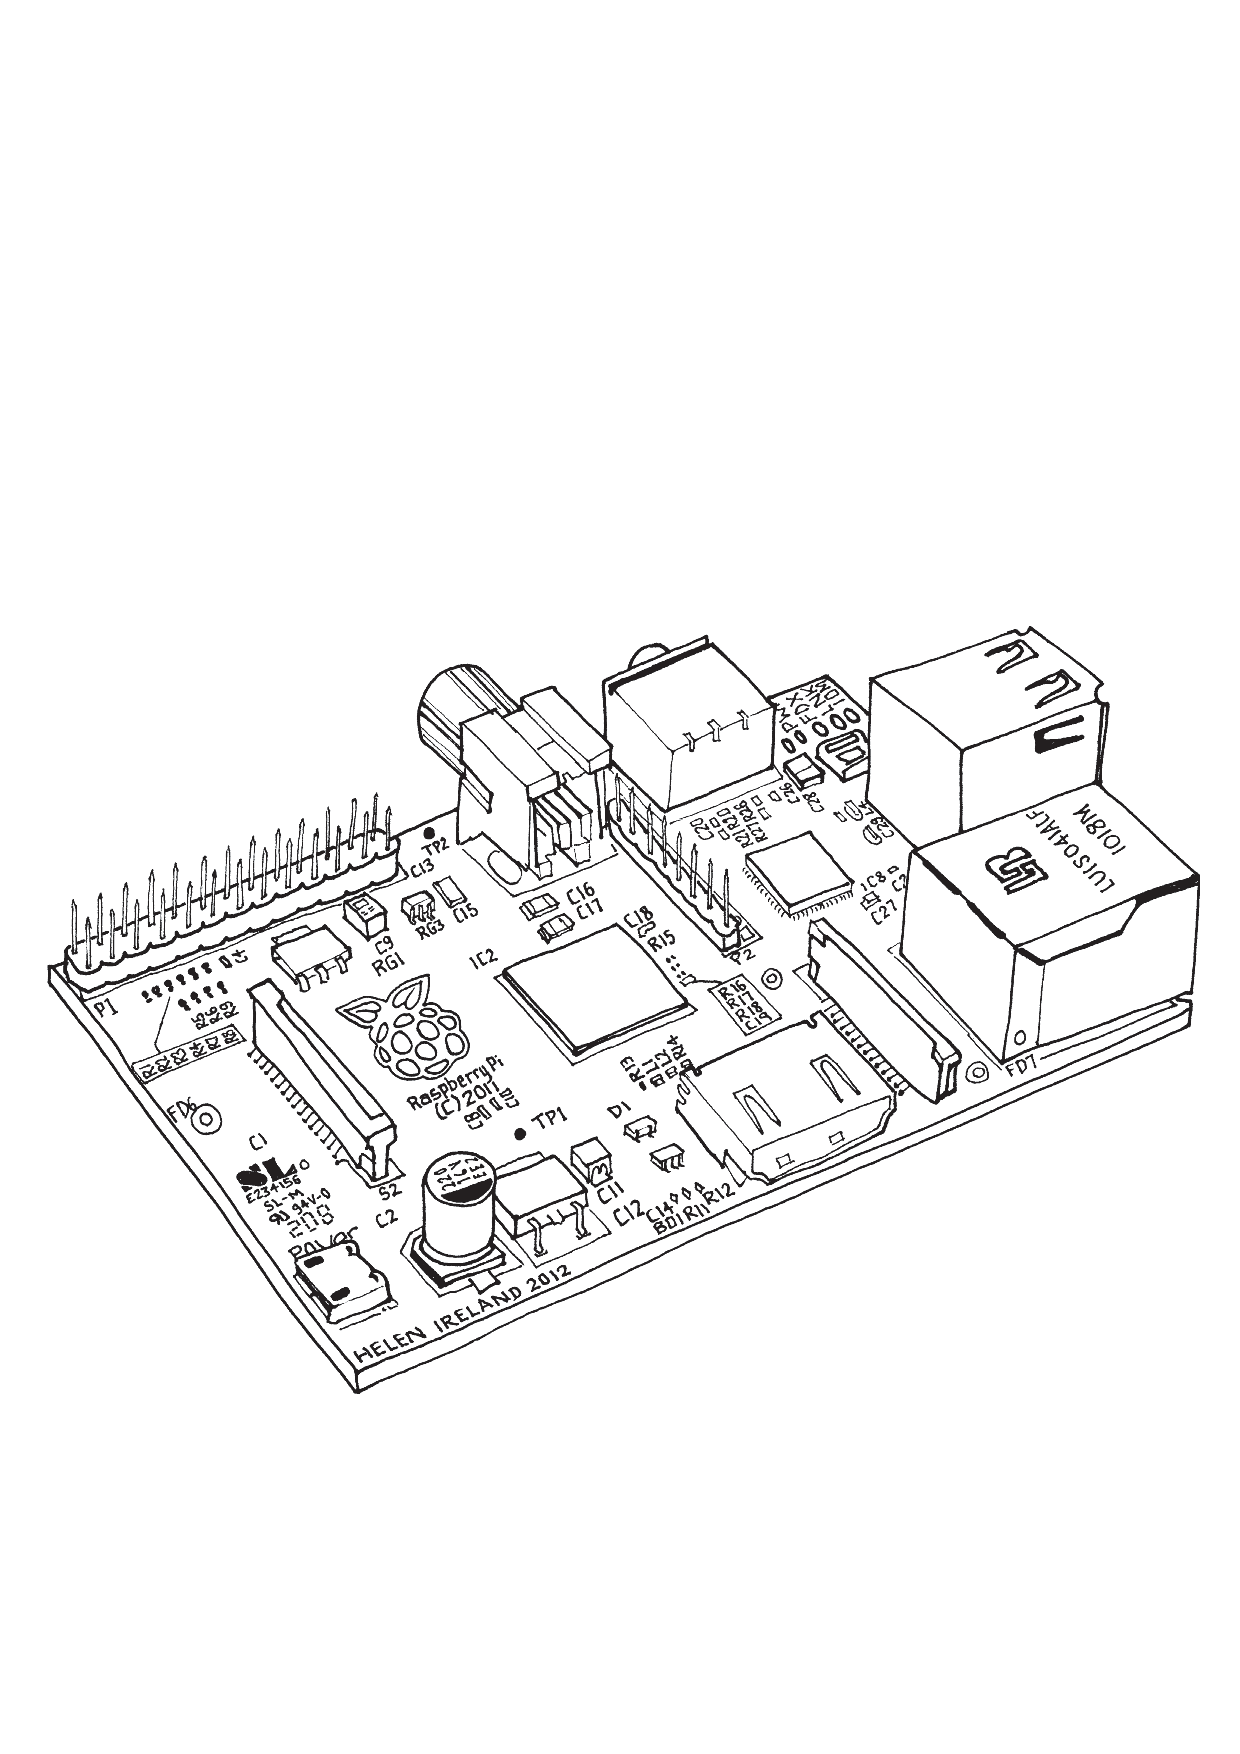
\includegraphics[width=0.7\textwidth]{rpi_grafik.pdf}\\ 
	\caption{Ein Raspberry Pi Modell B\cite{scrguide01}.}\label{fig:RPi-Spezifikation}
\end{figure}

\noindent Auf dieser Platine sind alle Komponenten verbaut, die den RPi zu einem voll funktionsf"ahigen Rechner machen: 

\subsection{SoC, CPU und GPU}\label{RPi Hardware}

Der RPi ist mit einem Broadcom BCM2835 als SoC ausgestattet. Es enth"alt die CPU (ein ARM1176JZFS-Prozessor) und die GPU (ein Broadcom VideoCore IV-Koprozessor)\footnote{Vgl. \cite{scrguide02}.}. Auff"allig ist, dass die CPU des RPi (ein ARM-Chip, wie er h"aufig in Mobiltelefonen verbaut ist), relativ schwach ist im Vergleich zur GPU, die Full HD-Aufl"osung und das hardwarebeschleunigte Rendern verschiedener Videoformate unterst"utzt. 

\subsection{Arbeitsspeicher}\label{RPi RAM}
Das Modell B des RPi verf"ugt "uber 512 MB SDRAM (gegen"uber dem Modell A mit 256 MB)\footnote{Vgl. ebd..}. Dieser kann nicht erweitert werden. Zu beachten ist aber, dass sich CPU und GPU den Arbeitsspeicher teilen und diese Einteilung durchaus ver"andert werden kann. Da der RPi kein BIOS hat, ist die einzige Zugriffsm"oglichkeit bzw. zur Allokation von RAM die Manipulation der Datei \verb+start.elf+ im Verzeichnis \verb+/boot+\footnote{Vgl. \cite{pow12}.}.

\subsection{Ausg"ange, Hauptspeicher und Stromversorgung}\label{RPi Schnittstellen}

Der RPi verf"ugt "uber einen HDMI-Ausgang, einen Cinch-Ausgang ("`RCA Jack"') und einen analogen Tonausgang. Er hat zwei USB 2.0-Schnittstellen und eine Ethernet-Schnittstelle. F"ur den nicht-fl"uchtigen Speicher ist eine SD-Speicherkarte vorgesehen, f"ur die ein Steckplatz vorhanden ist. Die Stromversorgung erfolgt "uber einen Mini-USB-Eingang. Zum Betrieb sind mindestens 700 mA/5 V n"otig\footnote{Vgl. \cite{pow12}.}. 

\subsection{GPIO/CSI}\label{RPi GPIO} 

Der RPi hat eine GPIO mit 6 Anschl"ussen, die jeweils "uber 26 Pins verf"ugen. "Uber die GPIOs k"onnen LEDs, Sensoren, Displays und andere Ger"ate angesteuert werden. I.d.R. wird dazu der GPIO-Connector P1 verwendet. Zur Steuerung der GPIOs existieren Bibliotheken f"ur verschiedene Programmiersprachen wie C, C++ und Python. Sie k"onnen auch "uber ein Terminal oder Web-Interfaces wie WebIOPi angesprochen werden. 

% evtl. Quelle ergänzen 

\subsection{Betriebssystem}\label{RPi OS}

F"ur den RPi existieren mehrere Implementierungen bzw. Derivate verbreiteter Betriebssysteme, darunter RISC OS und Plan 9. Am verbreitetsten sind Linux/Unix-basierte Systeme wie FreeBSD und NetBSD (BSD-Varianten), Raspbian (Debian-Variante), Pidora (Fedora-Variante) oder eine Variante von Arch Linux\footnote{Vgl. ebd..}.   

\section{Raspberry Pi-Cluster als Testumfeld}\label{Spezifikation Bramble}

In den letzten Monaten zeigte sich verst"arkt die Tendenz, eine gr"o\ss ere Anzahl von Raspberry Pis zu einem Cluster zu koppeln\footnote{Weitere Cluster-Projekte werden z.B. in \cite{cox13}, \cite{kie01}, \cite{bal12} und \cite{ou13} dargestellt.}. Im Folgenden wird die hier verwendete Architektur kurz vorgestellt\footnote{F"ur eine detaillierte Beschreibung vgl. \cite{kli13}.}. 

\subsection{Aufbau}\label{Bramble Hardware}
Der RPi-Cluster besteht aus 20 RPi Modell B-Einzelrechnern, die jeweils mit einem Ethernet-Kabel mit einem zentralen x86-Server (bestehend haupts"achlich aus einem Mini-ITX-Mainboard und einer Gigabit Ethernet-Netzwerkkarte) verbunden sind. Sie befinden sich in einem modifizierten Tower-Metallgeh"ause, das auf die Seite gedreht und oben offen gelassen wurde. Darin sind au\ss erdem ein 24 Port Gigabit-Switch, die Stromversorgung des Servers und der RPis sowie die K"uhlung integriert\footnote{Ein solches System relativ kosteng"unstiger Rechnermit einem BSD- oder Linux-Betriebssystem, die "uber IP kommunizieren, wird im Allgemeinen als \textit{Beowulf} bezeichnet (vgl. \cite{kie01} und \cite{kli13}). H"aufig dient es dem Ersatz oder der Simulation eines Supercomputers. Im Zusammenhang mit RPis ist auch der Begriff \textit{Bramble} gebr"auchlich, der im Folgenden verwendet wird (vgl. \url{www.raspberrypi.org/archives/tag/bramble}).}. 
% TODO Cluster fotografieren und Bild einbinden 
\begin{figure}[htb]
	\centering
	\includegraphics[width=0.7\textwidth]{bramble.pdf}\\ 
	\caption{Der hier verwendete Bramble.}\label{fig:Bramble}
\end{figure}

% NIC = Network Interface Card 

\subsection{Betriebssystem und Filesystem}\label{Bramble Systemarchitektur} 

Wie in Kap. \ref{RPi OS} beschrieben, existieren verschiedene Linux-Varianten f"ur den RPi. Als Betriebssytem f"ur den RPi-Einzelrechner und die Bramble-RPis wurde Raspbian, die offizielle Distribution der Raspberry Pi Foundation, gew"ahlt\footnote{Vgl. \url{http://www.raspberrypi.org/faqs}. Das verwendete Image findet sich unter \url{http://downloads.raspberrypi.org/raspbian_latest}.}. Auf den Einsatz von NOOBS\footnote{Die Raspberry Pi-Foundation empfiehlt besonders f"ur Einsteiger die \textit{New Out Of Box Software} und bietet entsprechend pr"aparierte SD-Karten zum Kauf an (vgl. \url{http://www.raspberrypi.org/archives/tag/noobs}).} oder anderer zus"atzlicher Bootloader wurde verzichtet\footnote{In diesem Fall fungiert die ausf"uhrbare Datei \texttt{start.elf}, die nach einer ausf"uhrbaren Datei \texttt{kernel.img} sucht und diese l"adt, als Bootloader (vgl. \cite{kli13}).}. Auf dem Server selbst l"auft eine Standard-Debian-Version. 

Ein Charakteristikum eines Beowulf-Clusters bzw. Bramble ist, dass es im Gegensatz zu einem "`richtigen"' Supercomputer kein Shared Memory-Interface und keine Cache-Koh"arenz gibt. Die Kommunikation zwischen den einzelnen Komponenten via Ethernet ist zudem relativ langsam. Es stellt sich daher die Frage nach dem Filesystem und der Synchronisierung der einzelnen Nodes. 

Um das Filesystem der einzelnen Nodes mit dem NFS des Servers zu synchronisieren, wurde hier eine Read-Only-Schicht f"ur die Slaves (Nodes) und eine Read-Write-Schicht f"ur den Master (Server) verwendet\footnote{Vgl. ebd..}. Um trotzdem die M"oglichkeit des gemeinsamen Zugriffs der Nodes auf ein Speichermedium zu haben, wurde ein geshartes Verzeichnis \texttt{/srv} eingerichtet. 

\subsection{Zugriff}\label{Bramble Zugriff}

Welche M"oglichkeiten gibt es nun, verteilte Anwendungen auf dem Bramble auszuf"uhren bzw. "uberhaupt die einzelnen Komponenten anzusprechen? Bei einem RPi-Einzelrechner nutzt man normalerweise einen USB-Port und den HDMI-Ausgang als stdin bzw. stdout. Eine andere M"oglichkeit besteht darin, den RPi "uber den Ethernet-Port mit einem Router zu verbinden und via SSH aus dem Intranet darauf zuzugreifen\footnote{Auf dem hier verwendeten Testger"at wurde letztere Variante gew"ahlt. Der Grund hierf"ur sind bekannte Probleme beim Anschluss "alterer Monitore oder Fernseher ohne HDMI-Eingang (vgl. z.B. \url{http://www.raspberrypi.org/forum/viewtopic.php?f=91&t=34061}).}. 

Der Zugriff auf den Bramble erfolgt ebenfalls aus dem internen Netzwerk via IP und SSH. Da sich die Architekturen des Servers und der RPi-Nodes unterscheiden, ist die einzige M"oglichkeit, auf diese zuzugreifen, wiederum via IP und SSH. Es gibt auf jedem RPi den Raspbian-Standard-User \texttt{pi}, der hier nicht ver"andert wurde\footnote{Auf dem RPi-Einzelrechner wurden aus Sicherheitsgr"unden Username und Passwort f"ur den Standard-User ge"andert.}. Um z.B. auf das gesharte Verzeichnis \texttt{/srv} zuzugreifen, sind \texttt{root}-Rechte erforderlich. 
\endinput 

	\chapter{Versuchsaufbau und -ablauf}\label{Kap3}

Das folgende Kapitel beschreibt Versuchsaufbau und -durchf"uhrung sowie Ziele der Messung, von der Erkenntnisse "uber das Skalierungsverhalten eines RPi-Clusters unter der Arbeitslast der ausgew"ahlten HPC-Benchmarks erwartet werden. 

\section{Zielsetzung}\label{Ziel}

F"ur das Skalierungsverhalten des Bramble unter der Arbeitslast von Linpack und STREAM werden wie in Kap. \ref{Kap2} beschrieben zwei Ma\ss zahlen betrachtet: Performance und Energieverbrauch.

Die augew"ahlten Benchmarks werden auf n -- 1 RPi-Knoten des Bramble mit n=19 RPi-Nodes ausgef"uhrt (vgl. Kap. \ref{Versuchsaufbau}). Alle Messungen werden zweimal durchgef"uhrt: Mit Stromanschluss der nicht beteiligten RPi-Nodes und ohne. F"ur beide Benchmarks werden zwei Ergebnisparameter betrachtet: Ausf"uhrungsrate in GFLOPs und Ausf"uhrungszeit in s f"ur HPLinpack, Ausf"uhrungsrate in MB/s und durchschnittliche Ausf"uhrungszeit in s f"ur STREAM. Die Ergebnisse der Messreihen werden anschlie\ss end gegen"ubergestellt (vgl. Kap. \ref{Ergebnisse}). 

\section{Aufbau und Art der Messung}\label{Aufbau}

Hier stellen sich zwei grunds"atzliche Fragen: Welcher Art ist die Messung und welche Voraussetzungen m"ussen hierf"ur erf"ullt sein? 

Die Performance wird pro Benchmark durch zwei Ergebnisparameter ermittelt. Zwei Messreihen werden durchgef"uhrt: Bramble mit n RPi-Knoten aktiv/20 RPi-Knoten angeschaltet, Bramble mit n RPi-Knoten aktiv/n RPi-Knoten angeschaltet. 
% TODO: evtl. bessere Einleitung/Herleitung 
F"ur den Versuchsaufbau sind folgende Aspekte von Bedeutung: M"ogliche Modifikationen der RPi-Knoten, Zeitsynchronisation der RPi-Knoten, Skalierung der Messung auf n -- 1 RPi-Knoten, automatisierte Durchf"uhrung der Messung auf n -- 1 RPi-Knoten sowie Einlesen der Messwerte in eine geeignete Datenstruktur. 

\subsection{Versuchsaufbau Ri-Einzelrechner}\label{RPi-Versuchsaufbau}

Viele Nutzer stellen sich nach Inbetriebnahme eines RPi-Einzelrechners die Frage nach Swap-Speicher und "Ubertakten (vgl. \cite{pow12}). Beides liegt nahe, da das Modell B des RPi nur "uber 512 MB Arbeitsspeicher verf"ugt. Die CPU-Leistung ist mit 700 MHz ebenfalls eher niedrig. 

Im Praxisbetrieb wurde gezeigt, dass ein "Ubertakten der CPU auf bis zu 1 GHz gefahrlos m"oglich ist (vgl. z.B. \url{http://www.raspberrypi.org/introducing-turbo-mode-up-to-50-} \url{more-performance-for-free/}). Bei den hier verwendeten RPis wurde davon Abstand genommen, da es wenig zielf"uhrend erscheint, die Komponente zu manipulieren, deren Performance man durch Benchmarking evaluieren m"ochte\footnote{F"ur eine zuk"unftige Untersuchung w"are es interessant zu ermitteln, ob man den relativ hohen Stromverbrauch des Bramble bei Niedriglast (vgl. \cite{kli13}) durch Untertakten der einzelnen CPUs senken kann (vgl. Kap. \ref{Kap5}).} Allerdings gibt es bereits Ergebnisse f"ur Linpack 100 und Whetstone bei auf einem RPi-Einzelrechner bei "Ubertakten der CPU auf 1 MHz (vgl. \url{http://www.roylongbottom.org.uk/Raspberry\%20Pi\%20Benchmarks.htm}).

Zur Allokierung von Swap-Speicher auf dem RPi gibt es grunds"atzlich drei M"oglichkeiten: Swap-Datei, Swap-Partition oder zRAM. 

Das Betriebssystem Raspbian verwendet standardm"a\ss ig eine Swap-Datei \texttt{/var/swap} auf der SD-Karte (vgl. \url{http://raspberrypi.stackexchange.com/questions/70/how-to-set} \url{-up-swap-space}). Hierbei zeigen sich Probleme: Erstens k"onnen st"andige Schreibzugriffe auf Dauer die SD-Karte besch"adigen. Zweitens sind Schreibzugriffe darauf sehr langsam, was die Performance des Systems bei hoher Arbeitsspeicherlast beeintr"achtigen kann (vgl. \cite{pow12}). 

Das gilt auch f"ur die Allokierung einer auf Unix-Systemen "ublicherweise genutzten Swap-Partition, weswegen diese M"oglichkeit in der Praxis keine Rolle spielt. 

Eine weitere M"oglichkeit des Swapping ist die Verwendung von zRAM. Hierbei wird ein Teil des Arbeitsspeichers komprimiert und als Swap Space genutzt. Hierbei werden keine Zugriffe auf die SD-Karte notwendig (vgl. \cite{pow12}). 

% Die Swap-Datei kann mit dem Befehl \texttt{sudo update-rc.d dphys-swapfile remove} deaktiviert werden. 
Auf dem Bramble-Server war kein Swap-Speicher allokiert worden (vgl. \cite{kli13}). Trotz der beschriebenen Schwierigkeiten wird auf den RPi-Knoten ein gro\ss er Teil des Speichers auf den SD-Karten als Swap-Speicher genutzt, um die Nutzung von Programmen mit mehr Speicherbedarf zu erm"oglichen und das Netzwerk durch das Cachen h"aufig verwendeter Dateien zu entlasten (vgl. \cite{kli13}).  

\subsection{Versuchsaufbau Bramble}\label{Bramble-Versuchsaufbau}

Das Komponentendiagramm \ref{fig:Komponentendiagramm} zeigt den Versuchsaufbau pro Messreihe auf dem Bramble mit Stromversorgung, Netzanschluss und Strommessger"at als phyischen Komponenten und der MySQL-Datenbank als logischer Komponente. Eine Messreihe wird als \textit{ExperimentSuite} bezeichnet. 
\begin{figure}[htb]
  \centering
  \centerline{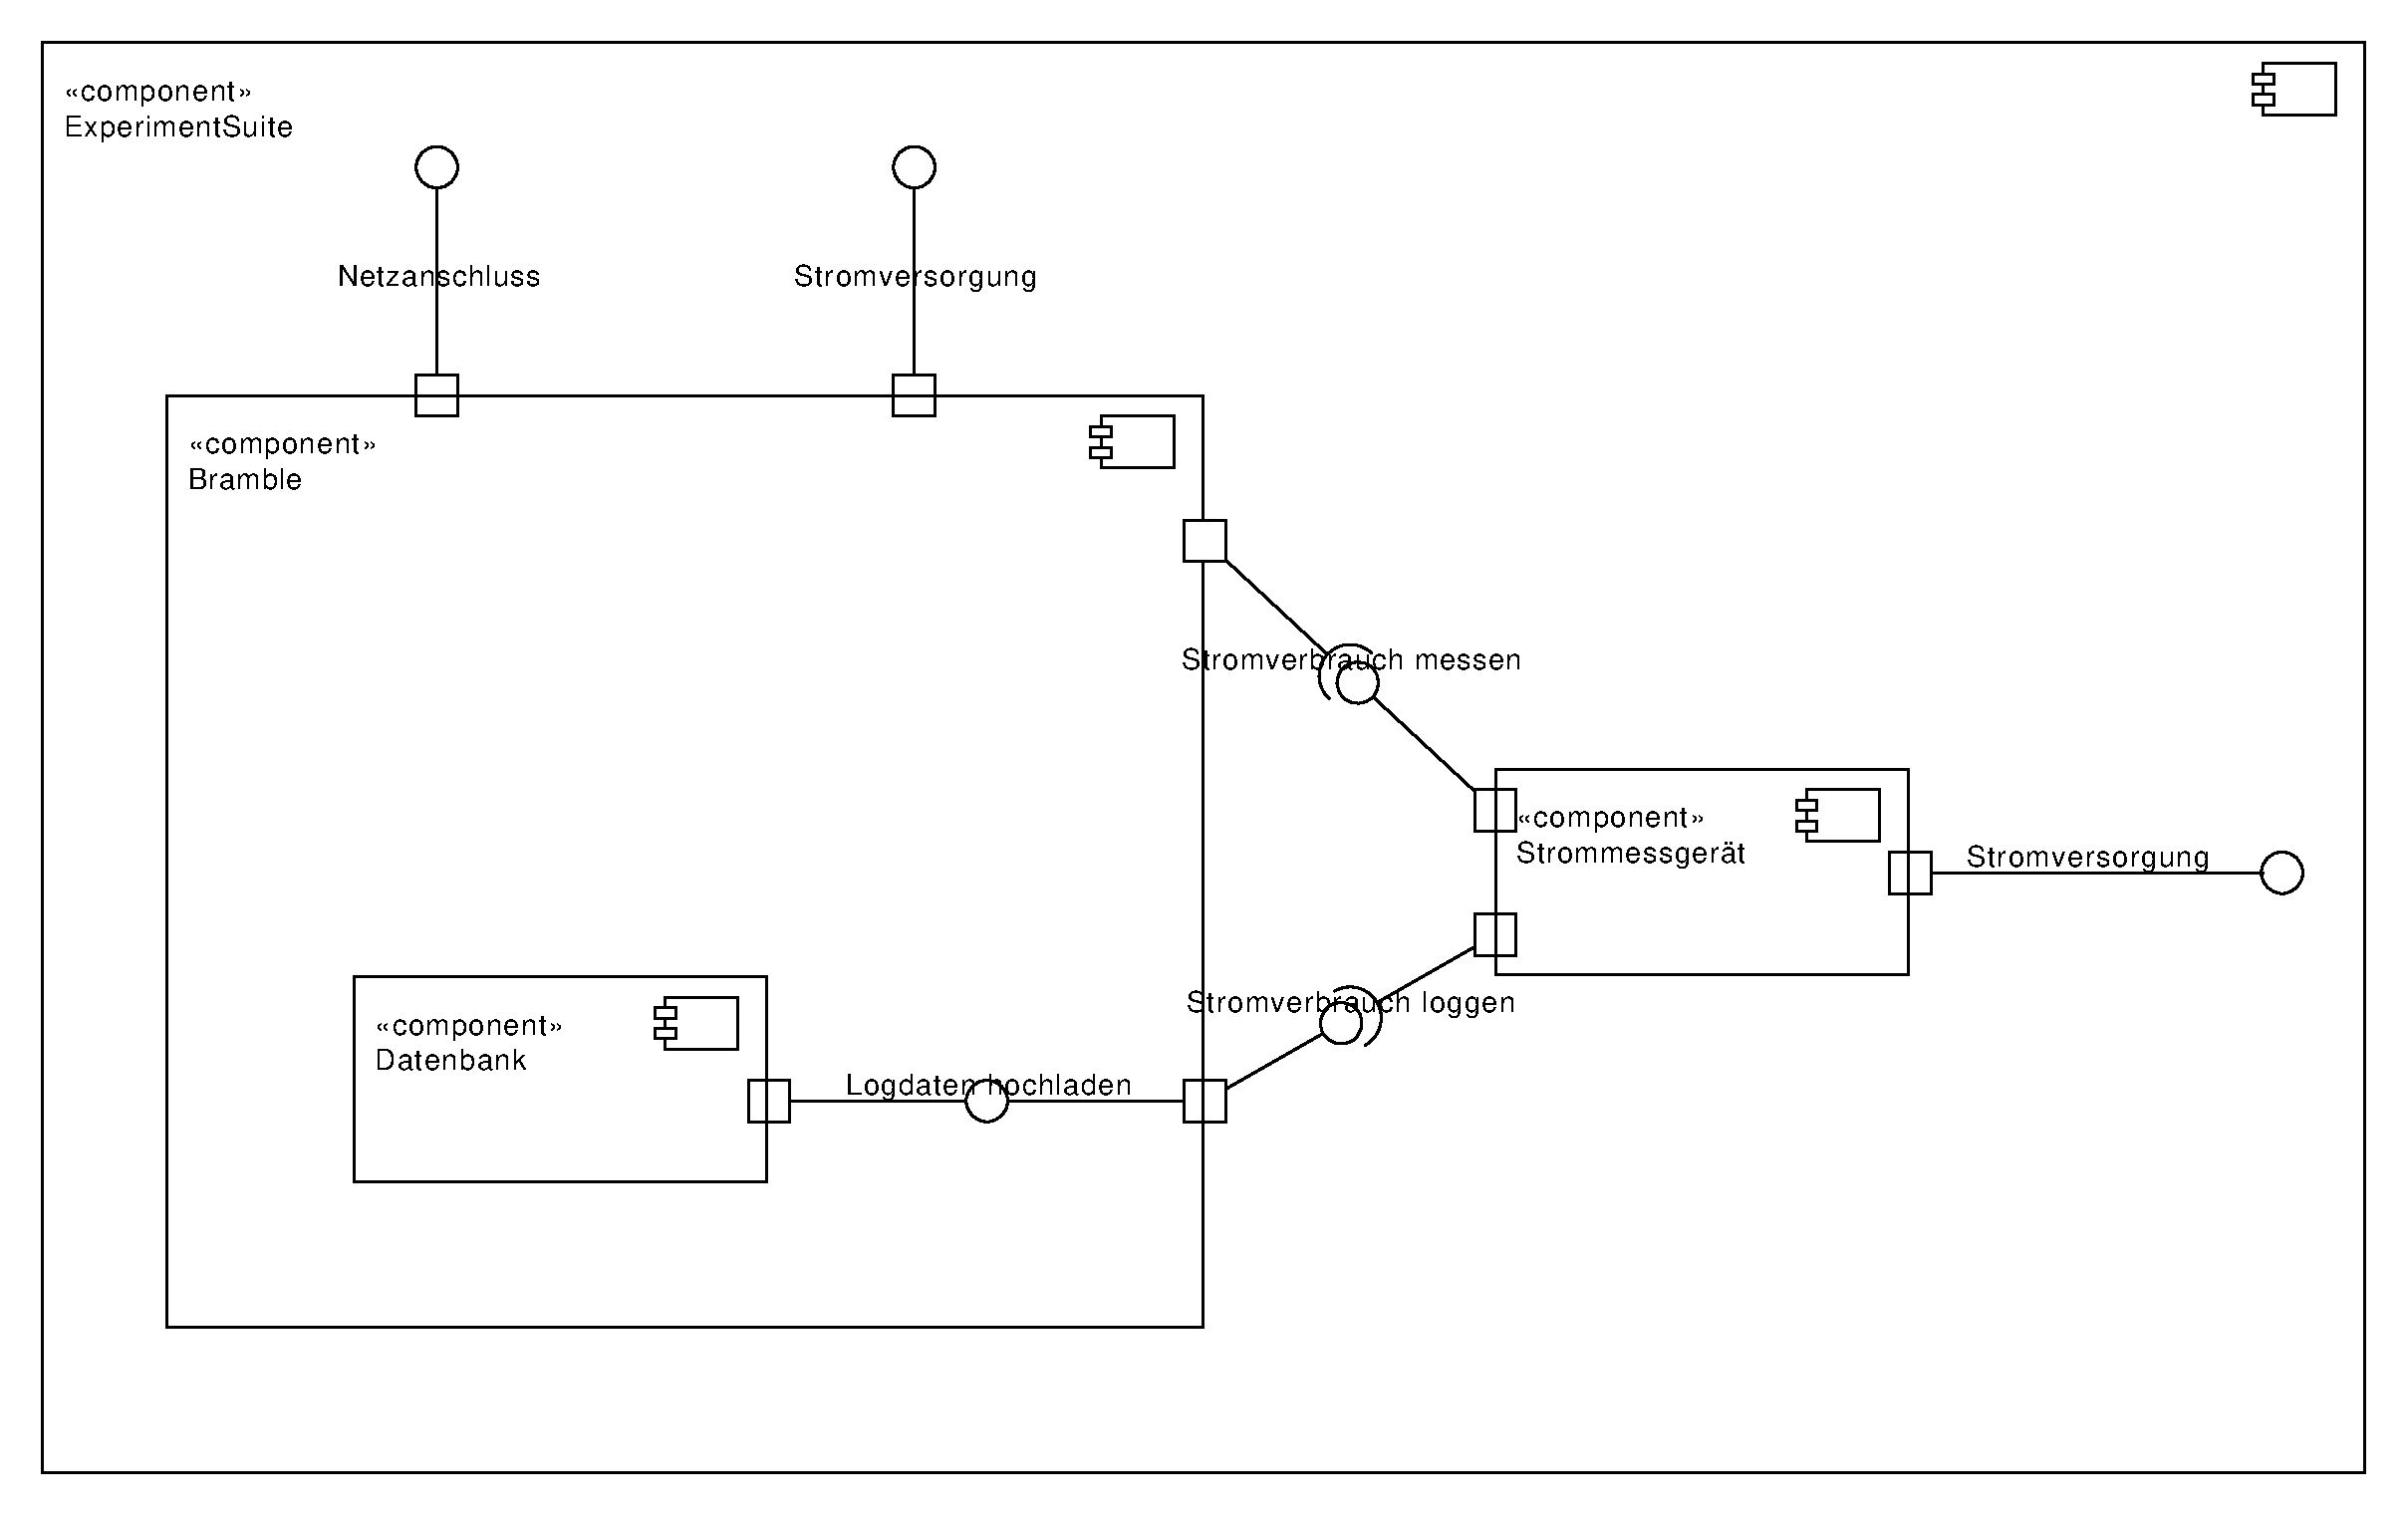
\includegraphics[scale=0.5]{komponentendiagramm2.pdf}} 
  \caption{Komponentendiagramm des Versuchsaufbaus.}
  \label{fig:Komponentendiagramm}		
\end{figure}
\subsubsection{Modifikation der RPi-Knoten}

Zu Beginn der Untersuchung zeigte sich, dass bei einige Mini-USB-Kabel zur Stromversorgung der RPis einen Wackelkontakt hatten oder ganz defekt waren. Um die in Kap. \ref{Vorgehensweise} genannte Zuverl"assigkeit des Versuchsaufbaus sicherzustellen, wurden sie durch funktionsf"ahige Kabel ersetzt. 

\subsubsection{Zeitsynchronisation der RPi-Knoten} 

Der RPi-Einzelrechner besitzt aus Kostengr"unden keine Systemuhr (vgl. \cite{schmi13}), sondern synchronisiert sich beim Booten gegen einen NTP-Server im Internet. F"ur die parallele Ausf"uhrung eines Programms auf mehreren Rechnerkernen ist die Zeitsynchronisation der RPi-Knoten und des Servers essentiell. Auf dem Bramble-Server gibt es daher einen OpenNTP-Server, gegen den sich die RPi-Knoten synchronisieren (vgl. \cite{kli13}). 

\subsubsection{Skalierung der Messung auf n -- 1 RPi-Knoten} 

Das Aktivit"atsdiagramm \ref{fig:Aktivitaetsdiagramm} zeigt, welche Schritte aus Benutzersicht f"ur die Durchf"uhr\-ung einer ExperimentSuite, d.h. der Ausf"uhrung eines Benchmarks auf einer gew"ahlten Anzahl aktiver und angeschalteter RPi-Knoten erforderlich sind. Es wird mit n=19 RPi-Knoten begonnen und einmal "uber alle Knoten von 19 -- 1 (ohne den Ausf"uhrungsknoten \texttt{pi03}) iteriert. Danach wird die zweite Messung durchgef"uhrt, wobei nach jedem Iterationsschritt der nicht mehr ben"otigte RPi-Knoten abgeschaltet wird. Jede Iteration der Benchmark-Ausf"uhrung l"auft prinzipell gleich ab, w"ahrend am Anfang und am Ende spezielle Vorkehrungen zu treffen sind. 
\begin{figure}[htb]
  \centerline{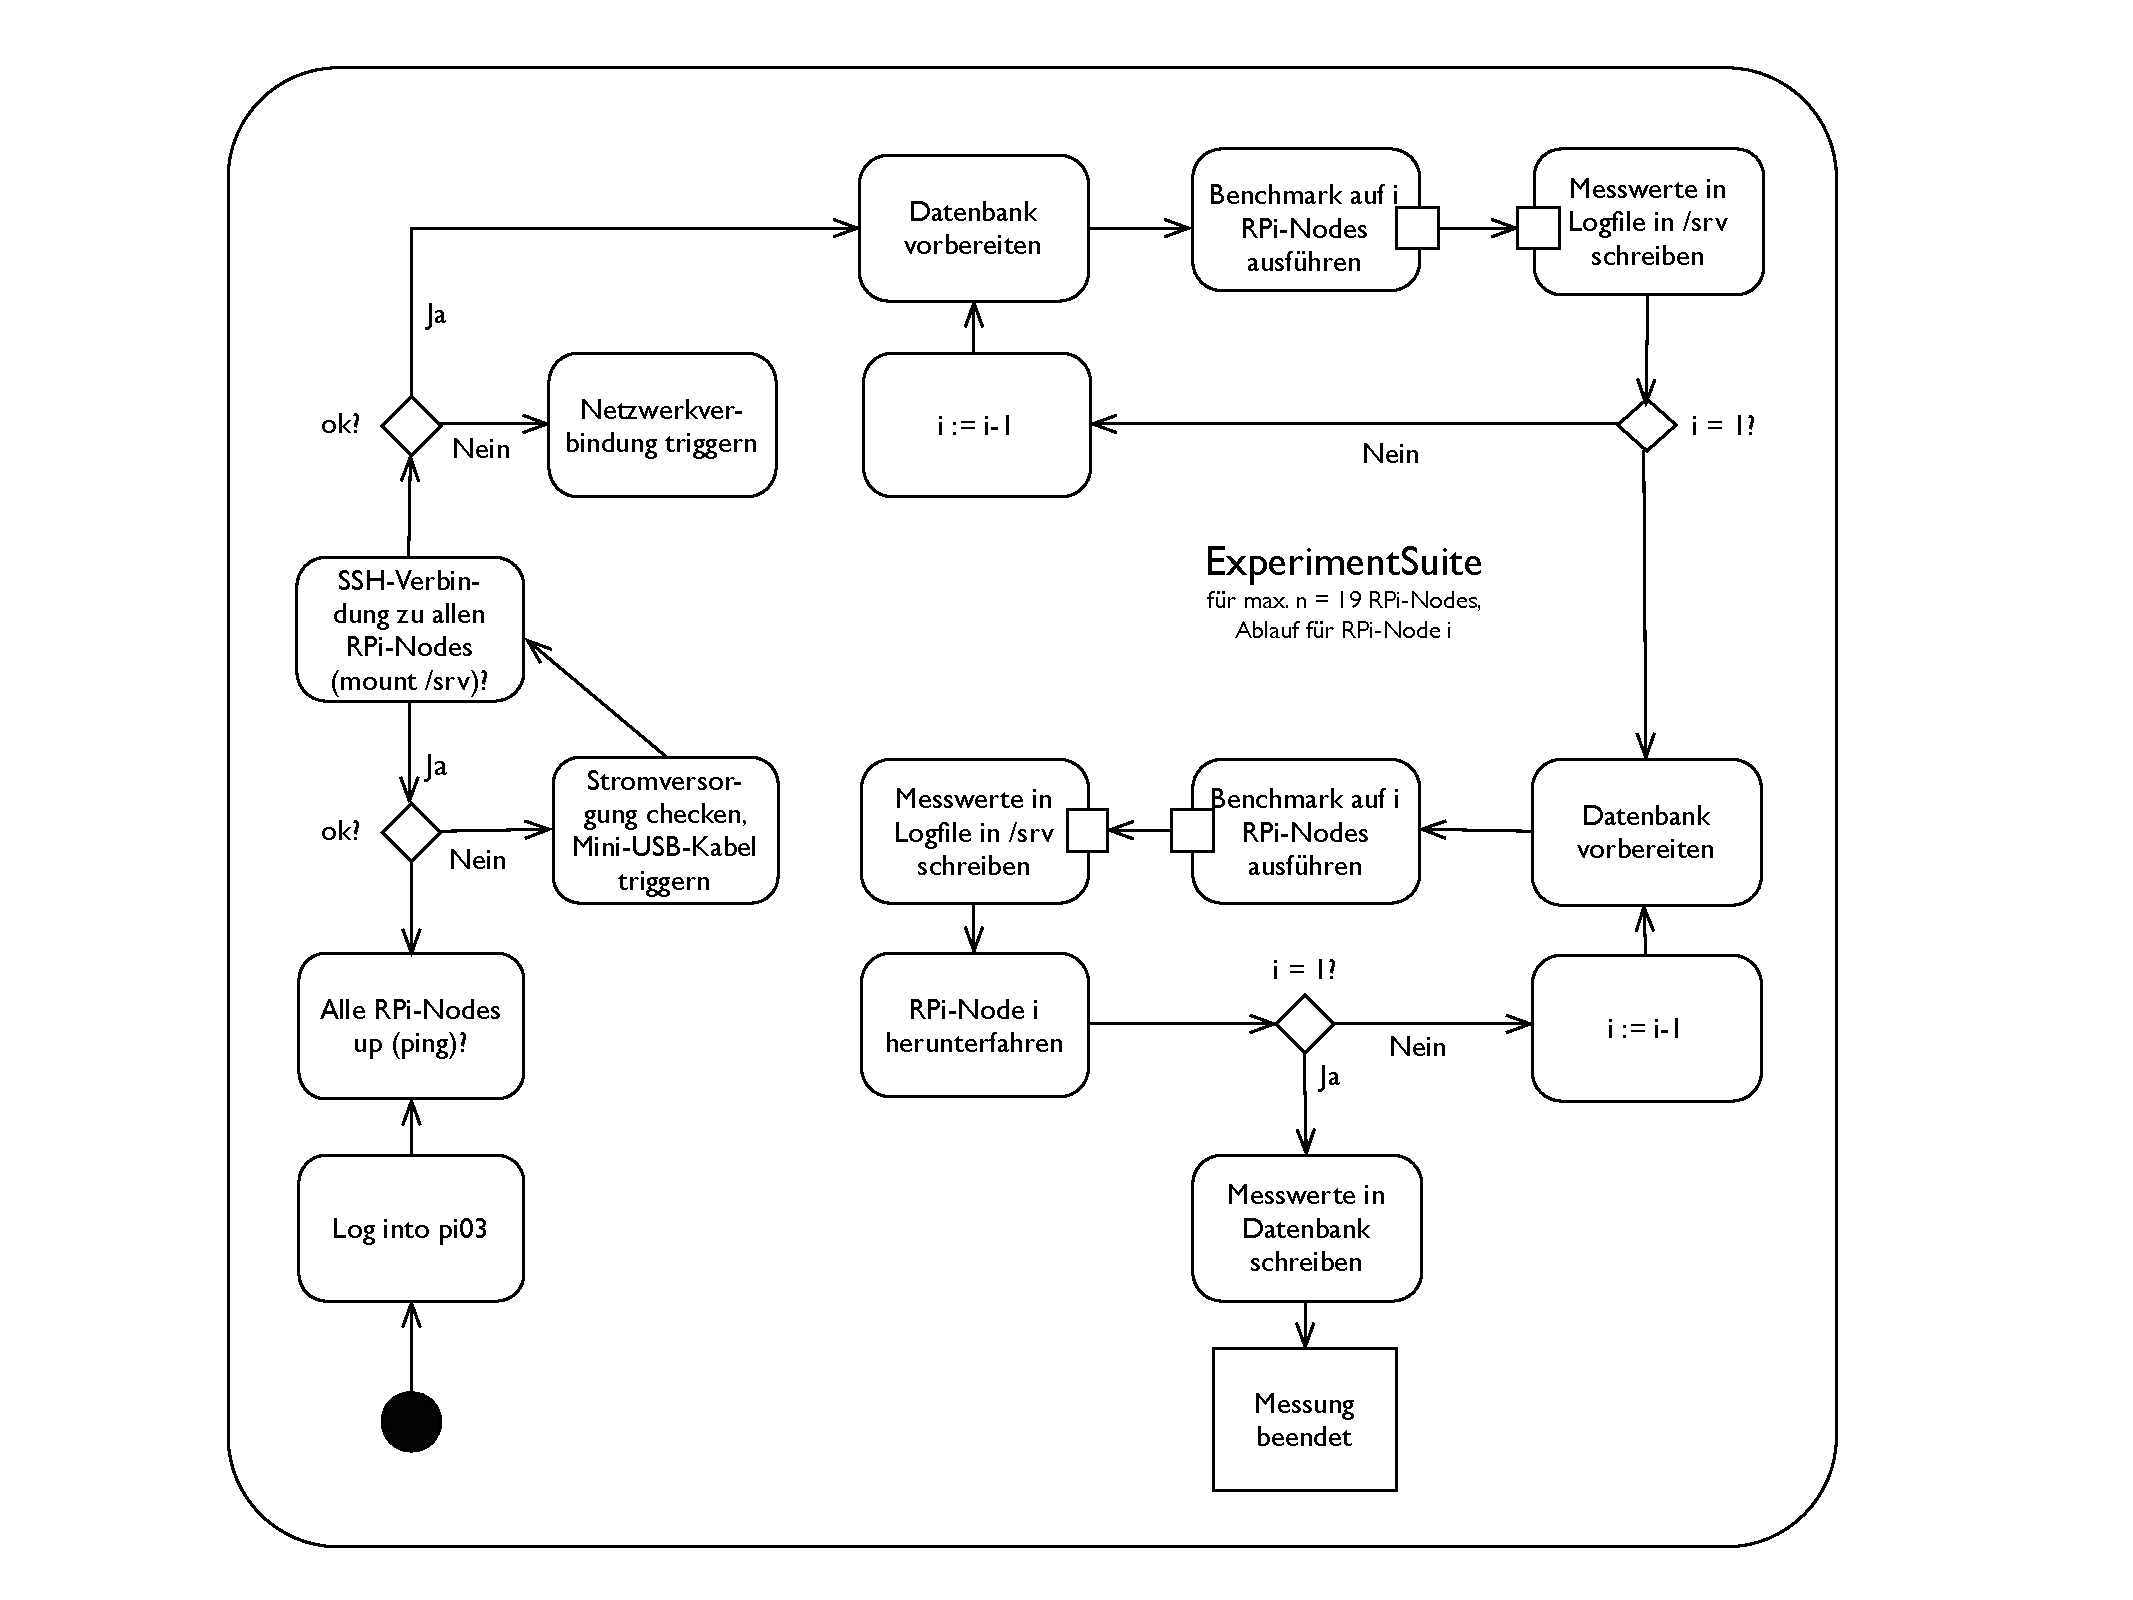
\includegraphics[scale=0.5]{aktivitaetsdiagramm1.pdf}} 
  \caption{Aktivit"atsdiagramm einer ExperimentSuite.}
  \label{fig:Aktivitaetsdiagramm}
\end{figure}

\subsubsection{Konfiguration der Datenbank}

Die Konfigurationen der Benchmarks und der ExperimentSuites sowie die Messergebnisse der Benchmarks werden in einer MySQL-Datenbank auf \texttt{careme} abgelegt. Daf"ur war ein Datenbankschema vorgegeben worden, das die Bramble-ExperimentSuites in einen gr"o\ss eren Versuchsaufbau integriert. W"ahrend der praktischen Arbeit wurde das Schema geringf"ugig an die tats"achlichen Erfordernisse angepasst. Z.B. wurde f"ur jedes ausgef"uhrte Teilmodul eines Benchmarks ein Messpaarameter definiert, der Unix-Timestamp seines Ausf"uhrungsendes ermittelt und zusammen mit dem jeweiligen Messwert in die Datenbank eingelesen.

Die Vorbereitung der Datenbank f"ur den Versuchaufbau erfolgt in vier Schritten:  
\begin{enumerate}\bfseries
	\item Name und Beschreibung des Benchmarks. 
	\item Beschreibung des Versuchsaufbaus. 
	\item Konfiguration des Versuchsaufbaus. 
	\item Verkn"upfung von Benchmark-Konfiguration und Versuchsaufbau.
\end{enumerate} 
Das Aktivit"atsdiagramm \ref{fig:Dbconfig1} visualisiert Schritt 1. Hier werden die statischen Konfigurationen f"ur STREAM und HPLinpack festgelegt, was durch zwei Shellskripte \texttt{loadGeneratorCon\-figHpl.sh} und \texttt{loadGenerator\-ConfigStream.sh} realisiert wird. Sie werden zu Beginn des Versuchs einmal ausgef"uhrt. Pro Benchmark muss in drei Tabellen jeweils ein Eintrag erstellt werden: In der Tabelle \texttt{LoadGenerator} muss ein Eintrag mit Werten f"ur Name und Beschreibung des Benchmarks eingegeben werden. In der Tabelle \texttt{ENUM\_LoadGeneratorConfigura\-tionKey} muss Eintrag mit einem Wert f"ur den Konfigurationsschl"ussel des Benchmarks erstellt werden. In der Tabelle \texttt{LoadGeneratorConfiguration} muss ebenfalls ein Eintrag mit diesem Wert erstellt werden.
\begin{figure}[htb]
\centering
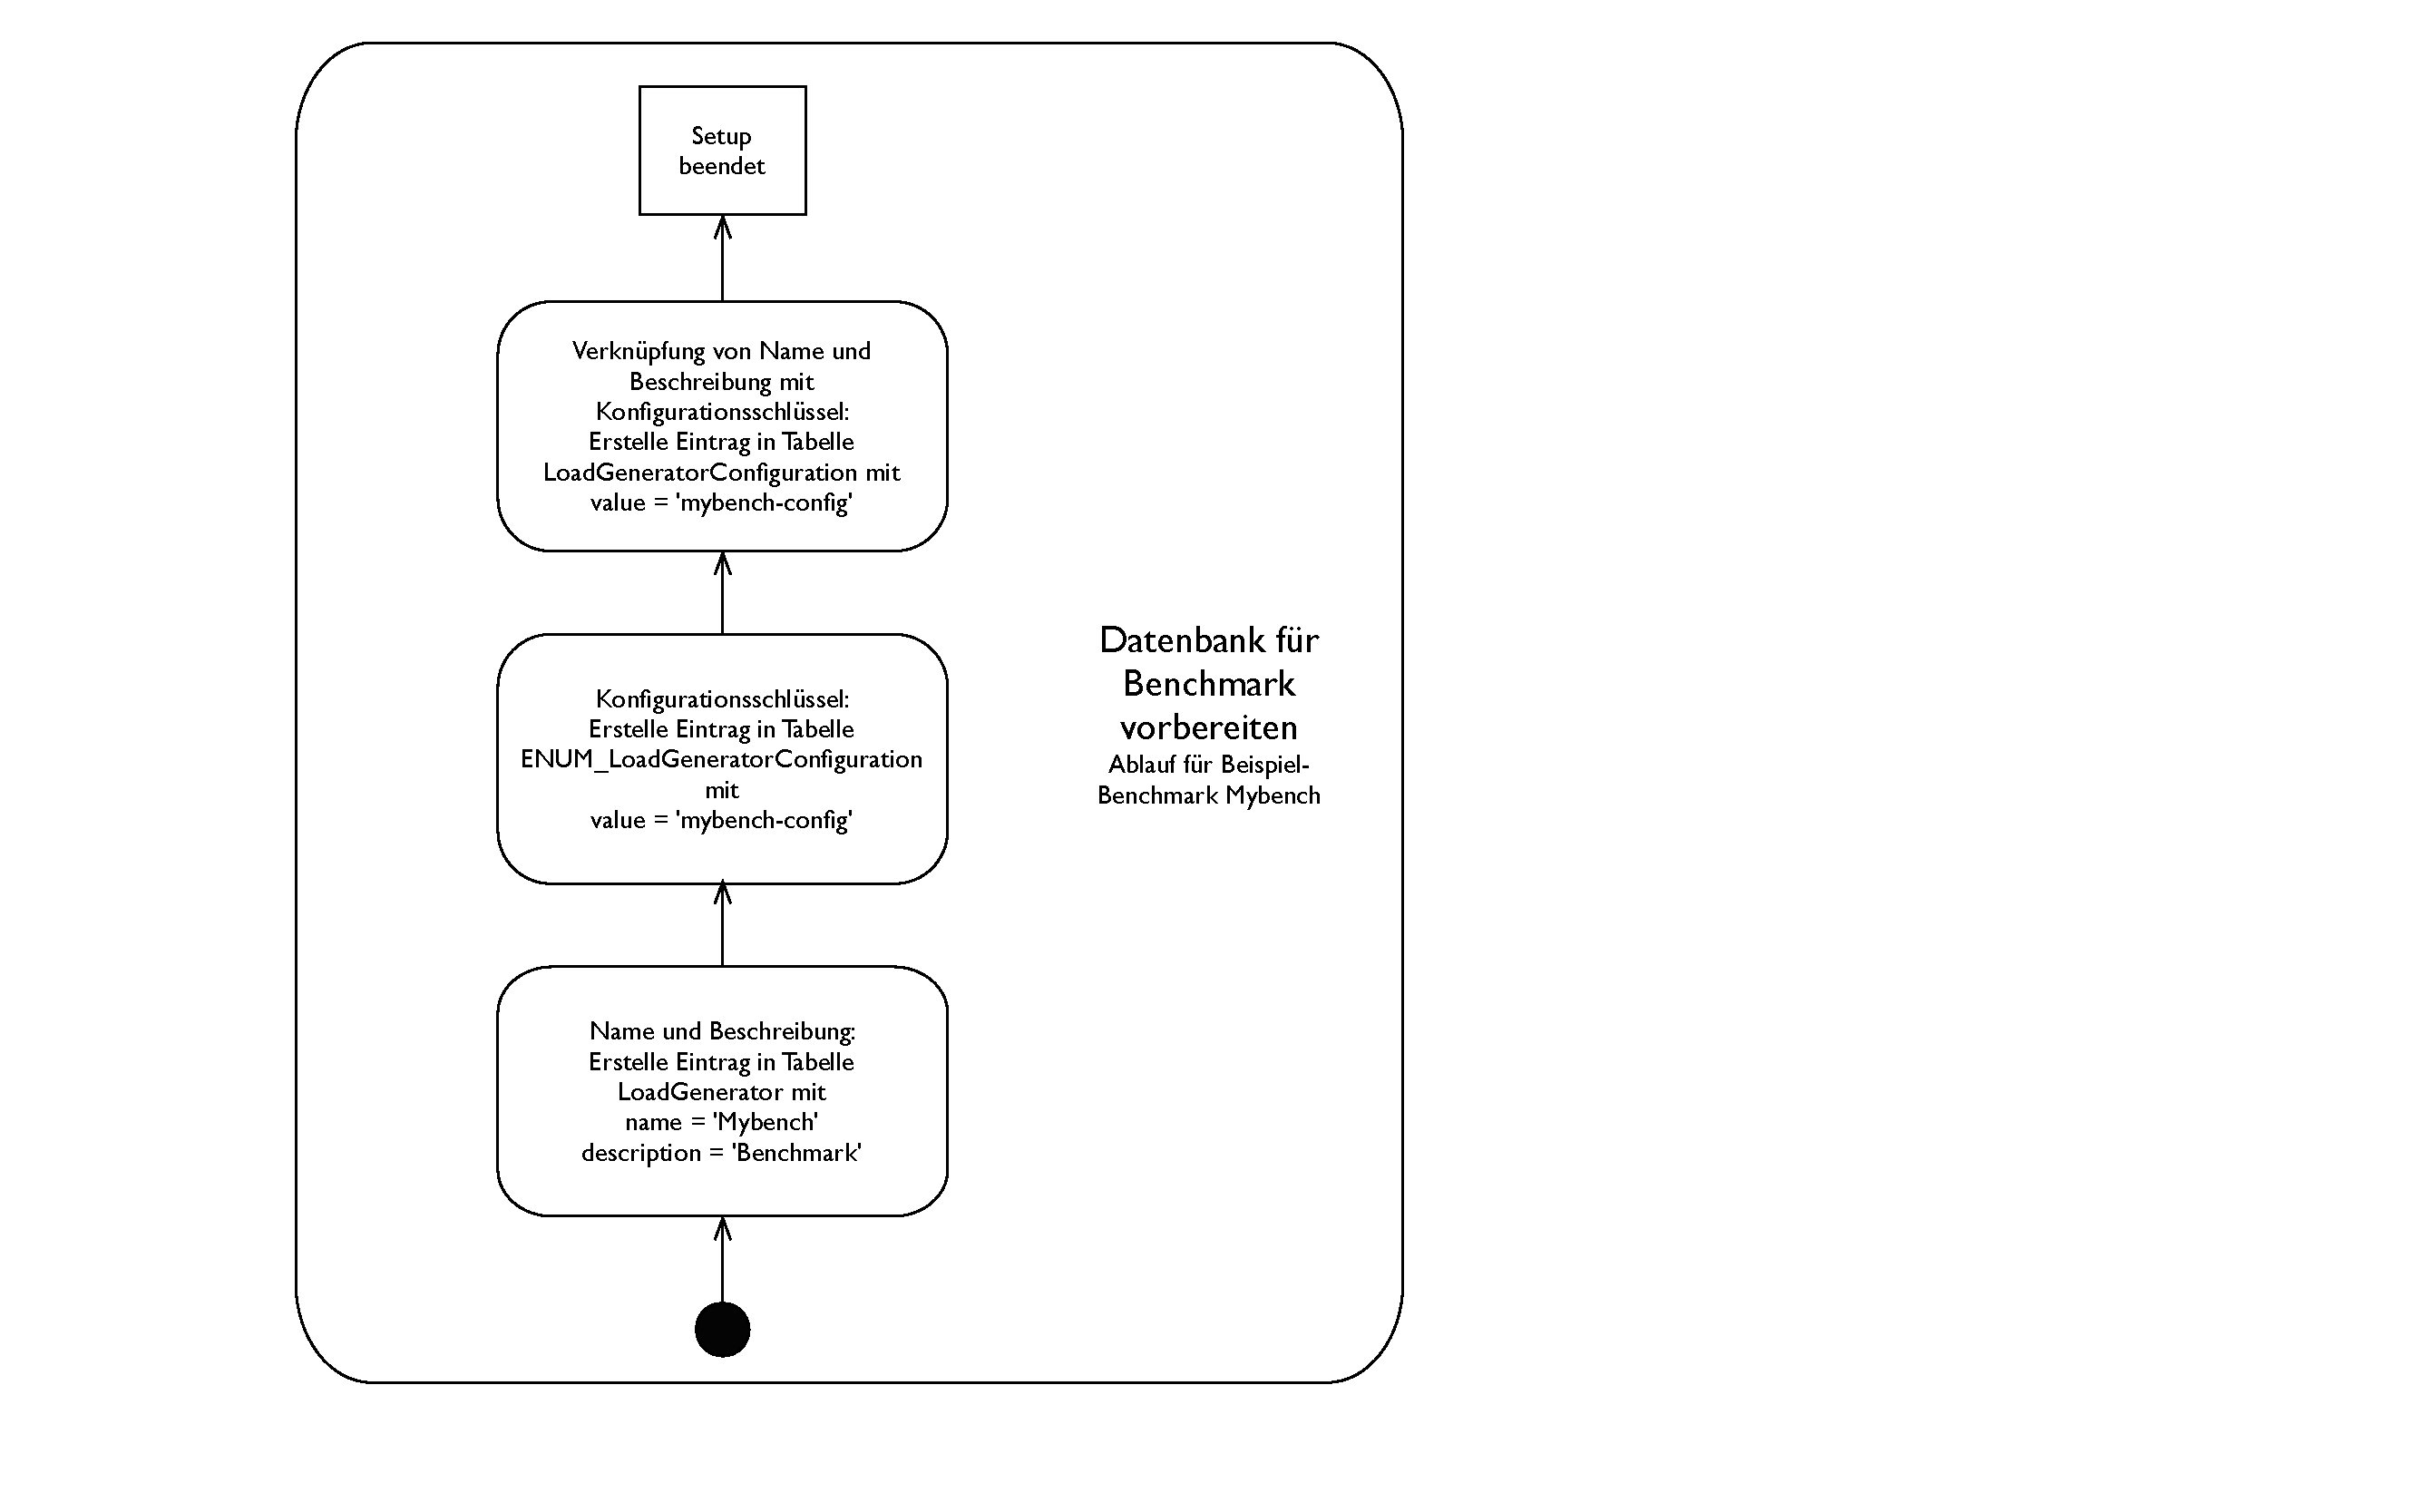
\includegraphics[scale=0.5]{dbconfig1.pdf}
\caption{Aktivit"atsdiagramm zur Vorbereitung der Datenbank f"ur einen Benchmark.}
\label{fig:Dbconfig1}
\end{figure}
Die dynamischen Schritte 2 -- 4, die pro ExperimentSuite ausgef"uhrt werden (Name, Beschreibung und Konfiguration des Versuchsaufbaus sowie Verkn"upfung von ExperimentSuite und Benchmark-Konfiguration) m"ussen pro Benchmark-Ausf"uhrung einmal erfolgen. Daher sind sie in die Ausf"uhrungsskripte f"ur die Benchmarks integriert, die im Folgenden dargestellt werden. Sie werden in Diagramm \ref{fig:Dbconfig2} veranschaulicht. 

\subsubsection{Automatisierte Durchf"uhrung der Messung auf n -- 1 RPi-Knoten} 

Die automatisierte Durchf"uhrung der Messung erfolgt durch Shellskripte. Sie werden im geteilten Verzeichnis abgelegt und k"onnen von \texttt{pi03} oder einem anderen Ausf"uhrungsknoten aus gestartet werden. Folgende Schritte werden durch die Skripte realisiert: 

\begin{enumerate}\bfseries
	\item Erstellen eines Machinefile zur Verteilung der Arbeitslast auf n RPi-Nodes, ggf. L"oschen des alten.\\
\normalfont{Der Aufruf von MPICH mit \texttt{mpiexec} zur verteilten Ausf"uhrung eines Programms auf mehreren CPUs erfolgt mit dem Parameter \texttt{-machinefile}. Damit wird auf die Datei verwiesen, in der die Reihenfolge der zu nutzenden CPUs und die Anzahl der darauf auszuf"uhrenden Prozesse angegeben ist. Ist eine CPU nicht verf"ugbar, weil z.B. der entsprechende RPi-Knoten heruntergefahren wurde, wird der Prozess auf der n"achsten verf"ugbaren CPU gestartet. 

Hierbei ist darauf zu achten, dass nur so viele Prozesse vergeben werden, wie auch angeschaltete RPi-Knoten zur Verf"ugung stehen. Die CPUs der RPi-Knoten m"ussen in der Reihenfolge angegeben werden, in der das Ausf"uhrungsskript das Herunterfahren der RPi-Knoten vorsieht. Das Machinefile muss in dem Verzeichnis abgelegt werden, von dem aus das auszuf"uhrende Programm gestartet wird. Um Verwechslungen vorzubeugen, wird ein eventuell dort liegendes, veraltetes Machinefile gel"oscht.}
	\textbf{\item Einh"angen des geteilten Verzeichnisses auf allen RPis.}\\
Alle die ExperimentSuites betreffenden Dateien, z.B. die ausf"uhrbaren Dateien der Benchmark-Programme und das Machinefile, liegen im geteilten Verzeichnis \texttt{/srv} bzw. \texttt{/srv/nfs-share}. Um sicherzustellen, dass ein Benchmark-Programm auf einem RPi-Knoten ausgef"uhrt werden kann, muss das geteilte Verzeichnis auf dem jeweiligen RPi-Knoten eingeh"angt sein. 
	\textbf{\item Navigation ins Arbeitsverzeichnis der ExperimentSuite.}\\
Alle Shellskripte zur Konfiguration und Ausf"uhrung der ExperimentSuites wurden in einem Verzeichnis \texttt{experimentsuite} im geteilten Verzeichnis \texttt{/srv} abgelegt. Die Ergebnisdaten werden ebenfalls dort abgelegt. 
	\textbf{\item Iteration "uber n ausgew"ahlte Benchmarks:}
	\begin{enumerate}\bfseries		
		\item Erstellen von Logdateien.\\
\normalfont{F"ur die Ergebnisse der Benchmarks werden Logdateien vorbereitet, in die sp"ater die Ausgabe der Benchmarks geschrieben wird.}  
		\textbf{\item Iteration "uber n RPi-Knoten:}
		\begin{enumerate}\bfseries
			\item Datenbank f"ur ExperimentSuite vorbereiten.\\ 
\normalfont{Das Aktivit"atsdiagramm \ref{fig:Dbconfig2} zeigt das Vorbereiten der Datenbank \texttt{rpiWerte} f"ur die aktuelle Iteration: F"ur jede Ausf"uhrung eines Benchmark-Programms muss ein Eintrag in der Tabelle \texttt{ExperimentSuite} mit Werten f"ur Granularit"at, Ziel und Startzeitpunkt erstellt werden. In der Tabelle \texttt{Experiment\-Suite\-Configuration} muss ein Eintrag mit Werten f"ur die Anzahlen aktiver und angeschalteter RPi-Knoten erstellt werden. Beide Tabellen werden "uber die Tabelle \texttt{N2M\_loadConf3expSuite} miteinander verkn"upft, in der ein Eintrag mit Werten f"ur  die ID des Benchmarks und die ID der ExperimentSuite erstellt werden muss.}
\begin{figure}[htb]
\centerline{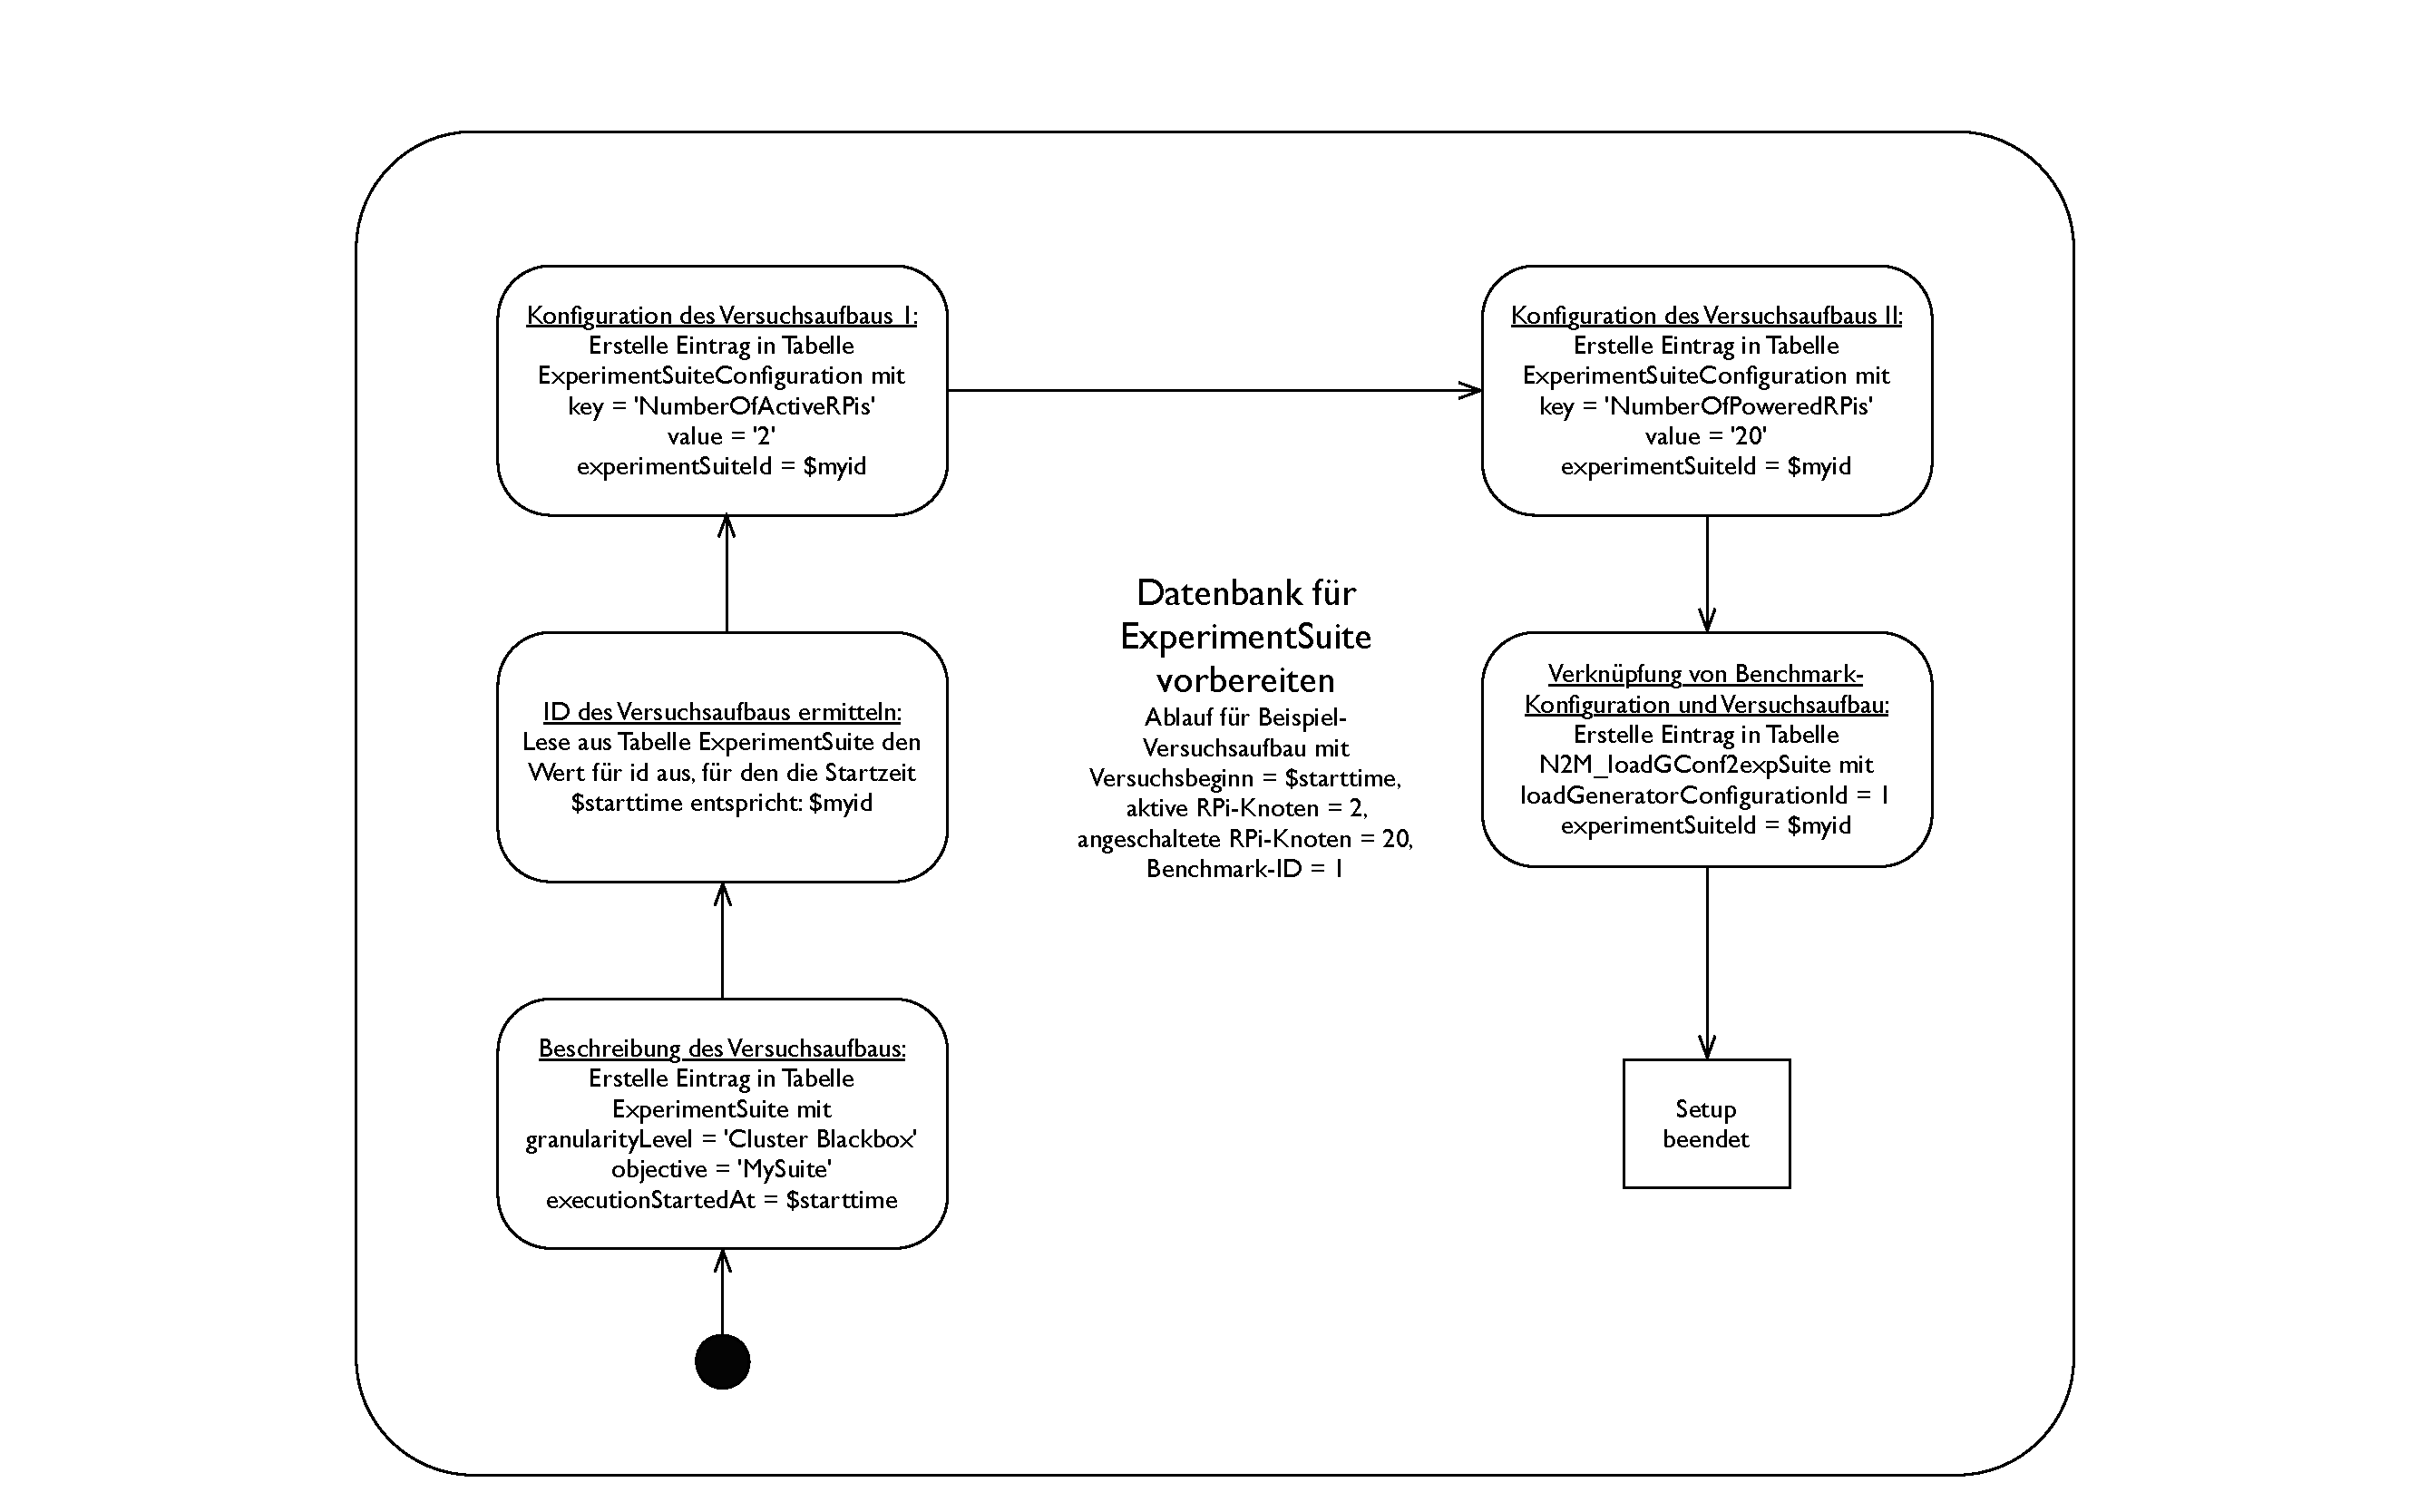
\includegraphics[scale=0.5]{dbconfig2.pdf}}
\caption{Aktivit"atsdiagramm zur Vorbereitung der Datenbank f"ur eine ExperimentSuite.}
\label{fig:Dbconfig2}
\end{figure}
			\textbf{\item Verteilte Ausf"uhrung des Benchmarks auf n RPi-Knoten.}\\ 
Die verteilte Ausf"uhrung eines Benchmark-Programms wird mit dem Befehl 
\begin{verbatim}
mpiexec -n -machinefile -wdir file 
\end{verbatim}
gestartet. Dabei spezifiziert \texttt{-n} die gew"unschte Anzahl an parallelen Programmaufrufen, \texttt{-machinefile} den Pfad zum Machinefile, \texttt{-wdir} das Verzeichnis, in das zur Ausf"uhrung des Programms gewechselt werden soll, und \texttt{file} die auszuf"uhrende Datei (vgl. \url{http://www.mpich.org/static/docs/latest/www1/mpiexec.html}). Ein Beispielaufruf zur parallelen Ausf"uhrung von HPLinpack auf vier RPi-Nodes mit der hier verwendeten Verzeichnisstruktur w"are also  
\begin{verbatim}
mpiexec -n 4 -machinefile /srv/libraries/etc/mpich-3.0.4-shared
/machinefile -wdir /srv/benchmarks/bin
/hpl-2.1 /srv/benchmarks/bin/hpl-2.1/xhpl
\end{verbatim}
			\textbf{\item Schreiben der Ergebnisdaten.}\\
Die Ausgabe des Benchmark-Programms wird in die vorbereitete Logdatei geschrieben. Falls das Programm in seiner Ausgabe keinen Zeitstempel vorsieht (z.B. STREAM), wird dieser ermittelt und der Ausgabe als zus"atzliche Zeile hinzugef"ugt. Das ist wichtig, damit sp"ater f"ur jeden Messwert ein Zeitstempel in die Datenbank eingegeben werden kann (vgl. Schritte d und e). Auch zum Abgleich der Messergebnisse der Benchmarks mit denen des Strommessger"ats ist ein Zeitstempel n"otig. % TODO: Verweis
		\end{enumerate}
		\textbf{\item Iteration "uber n RPi-Knoten:} 
		\begin{enumerate}\bfseries
			\item Einrichten der Datenbank.\\
\normalfont{Die Datenbank wird wie in Schritt b i beschrieben vorbereitet. Der wesentliche Unterschied zu Schritt ist der Wert f"ur die Anzahl angeschalteter RPi-Knoten. Es wird nicht mehr konstant 20 eingetragen, sondern n, da nicht mehr aktive RPi-Knoten heruntergefahren werden.} 
			\textbf{\item Verteilte Ausf"uhrung des Benchmarks auf n RPi-Knoten.}\\
Analog zu Schritt b ii.
			\textbf{\item Herunterfahren von RPi-Knoten n.}\\
Beim zweiten Lauf eines Benchmark-Programms auf n RPi-Knoten wird der nun nicht mehr ben"otigte bzw. aktive Knoten heruntergefahren. Das gilt nicht f"ur den Ausf"uhrungsknoten \texttt{pi03}, der bis zum Schluss des Experiments zur Ausf"uhrung der Skripte und Eingabe der Messergebnisse in die Datenbank verwendet wird. 
			\textbf{\item Schreiben der Ergebnisdaten.}\\ 
Analog zu Schritt b iii.
		\end{enumerate}
		\textbf{\item Parsen der Logdateien f"ur die Datenbank-Eingabe.}\\
Die Ausgabe der Benchmarks ist h"ochst unterschiedlich und entspricht nat"urlich nicht dem Eingabeformat f"ur die Datenbank \texttt{rpiWerte}. Daher wird pro ausgef"uhrtem Benchmark eine Eingabedatei f"ur die Datenbank erstellt, die pro ExperimentSuite eine Zeile mit den Messergebnissen und Zeitstempel enth"alt, getrennt durch Leerzeichen. So enth"alt z.B. eine Zeile einer Datenbank-Eingabedatei f"ur STREAM: 
\begin{verbatim}
Copy: 3649.3 0.167595 0.166607 0.168846 Scale: 3428.0 0.178749 
0.177361 0.180439 Add: 4749.8 0.192614 0.192010 0.193745 Triad: 
4630.1 0.197780 0.196974 0.199436 Unixtime: 1396608095
\end{verbatim} 
Eine Beispielzeile einer Datenbank-Eingabedatei f"ur HPLinpack: 
\begin{verbatim}
WR00L2L2 29 1 2 2 0.09 1.965e-04 HPL_pdgesv() end time Wed Mar 
26 15:39:05 2014
\end{verbatim} 
		\textbf{\item Schreiben der Messergebnisse in die Datenbank.}\\
Falls die Zeitstempel in der Datenbank-Eingabedatei noch nicht dem Format des Unix-Zeitstempels UTC entsprechen (vergangene Sekunden seit dem 1. Januar 1970, vgl. \url{http://unixhelp.ed.ac.uk/CGI/man-cgi?date}) wie z.B. bei HPLinpack (vgl. Schritt d), werden sie in dieses Format konvertiert. F"ur jeden Messwert muss ein Eintrag in der Tabelle \texttt{MeasurementValue} mit Werten f"ur Parameter, Messwert und Zeitstempel erstellt werden. 		
	\end{enumerate}
\end{enumerate}
\noindent
Zur Durchf"uhrung dieser Schritte wurden drei Shellskripte erstellt: \texttt{startBenchmarks.sh} zum Erstellen des Machinefile, Einh"angen des geteilten Verzeichnisses und Aufruf der Skripte \texttt{STREAM.sh} und \texttt{hpl-2.1.\-sh} (Schritte 1--3). Schritt 4 wird f"ur den jeweiligen Benchmark durch die Shellskripte \texttt{STREAM.sh} und \texttt{hpl-2.1.sh} ausgef"uhrt, die von \texttt{startBenchmarks.sh} aufgerufen werden. 

\section{Strommessung}
% Name, Beschreibung
Die Messung des Stromverbrauchs erfolgt mit dem Strommessger"at Energenie EGM-PWM-LAN (vgl. \url{http://energenie.com/item.aspx?id=6736&lang=de}), im Folgenden als \textit{Energenie} bezeichnet. Es wird zwischen die Steckdose und den Bramble gesteckt und "uber ein LAN-Kabel wird es mit dem Netzwerk verbunden. 

% Aktivierung
F"ur den hier verwendeten Versuchsaufbau war dem Energenie eine statische IP-Adresse zugewiesen und ein DNS-Eintrag f"ur es erstellt worden. Damit ist es m"oglich, im lokalen Netzwerk auf das Ger"at und die von ihm ermittelten Messwerte zuzugreifen. Dazu bietet das Energenie mehrere M"oglichkeiten, darunter eine Webbrowser-Oberfl"ache und ein Windows-Programm. Damit die Software das Ger"at erkennt, muss es sich im selben Subnetz befinden wie der Rechner, von dem aus der Zugriff erfolgt.  

% Datenspeicherung 
Das Energenie misst Spannung in Volt, elektrischen Strom in Ampère, Leistung in Watt und Arbeit in Kilowattstunden. Die Messgenauigkeit betr"agt dabei $+/- 2\% bzw. +/- 1 W$ innerhalb des Messbereichs von 50 W -- 2500 W. % TODO Messfehler ermitteln 

% Datenzugriff 
F"ur den Versuchsaufbau erwies sich die Webbrowser-Oberfl"ache als weniger geeignet, da sie haupts"achlich Konfigurationsfunktionen bietet. Zwar werden auf einer grafischen Oberfl"ache die jeweils aktuellen Werte f"ur Spannung in Volt, elektrischen Strom in Ampère, Leistung in Watt und Arbeit in Kilowattstunden angezeigt, doch es k"onnen keine Messwerte "uber eine Zeitspanne abgerufen werden. Das Windows-Programm bietet erweiterte Funktionalit"aten, z.B. die Visualisierung der Leistung "uber eine Zeitspanne als als Kurve.  

Bei Verwendung der Software \textit{PowerManager} werden die Messwerte in der SQLite-Datenbank \texttt{database.sqlite} im Verzeichnis \texttt{C:\textbackslash Program Data\textbackslash PowerManagerDatabase} auf der zugreifenden Windows-Maschine abgelegt. Die Messwerte k"onnen auch als xls-Datei exportiert werden. Dabei Drei werden pro Messung drei Werte angegeben: Beginn der Aufzeichnung, Ende der Aufzeichnung und Leistung in Watt. In der Datenbank werden f"ur jede Messung zus"atzliche Werte abgelegt wie Widerstand in Ohm und Frequenz in Hertz. Die f"ur die ExperimentSuite wichtigen Messwerte sind die Eintr"age f"ur \texttt{Stamp} (Zeitstempel als Integer-Wert) und \texttt{P} (Leistung in Watt als Double-Wert), die in der Tabelle \texttt{LogValues}. Die Entscheidung f"ur das Auslesen der SQLite-Datenbank gegen"uber dem xls-Export fiel wegen der h"oheren Granularit"at der Zeitstempel. 

% Setup für ExperimentSuite 
Das Aktivit"atsdiagramm \ref{fig:energenie} visualisiert die Schritte, die pro ExperimentSuite notwendig sind, um Messwerte f"ur den Stromverbrauch zu generieren, auszulesen und den Messwerten der Benchmark-Programme gegen"uberzustellen: 
%\begin{figure}[htb]
%  \centering
%  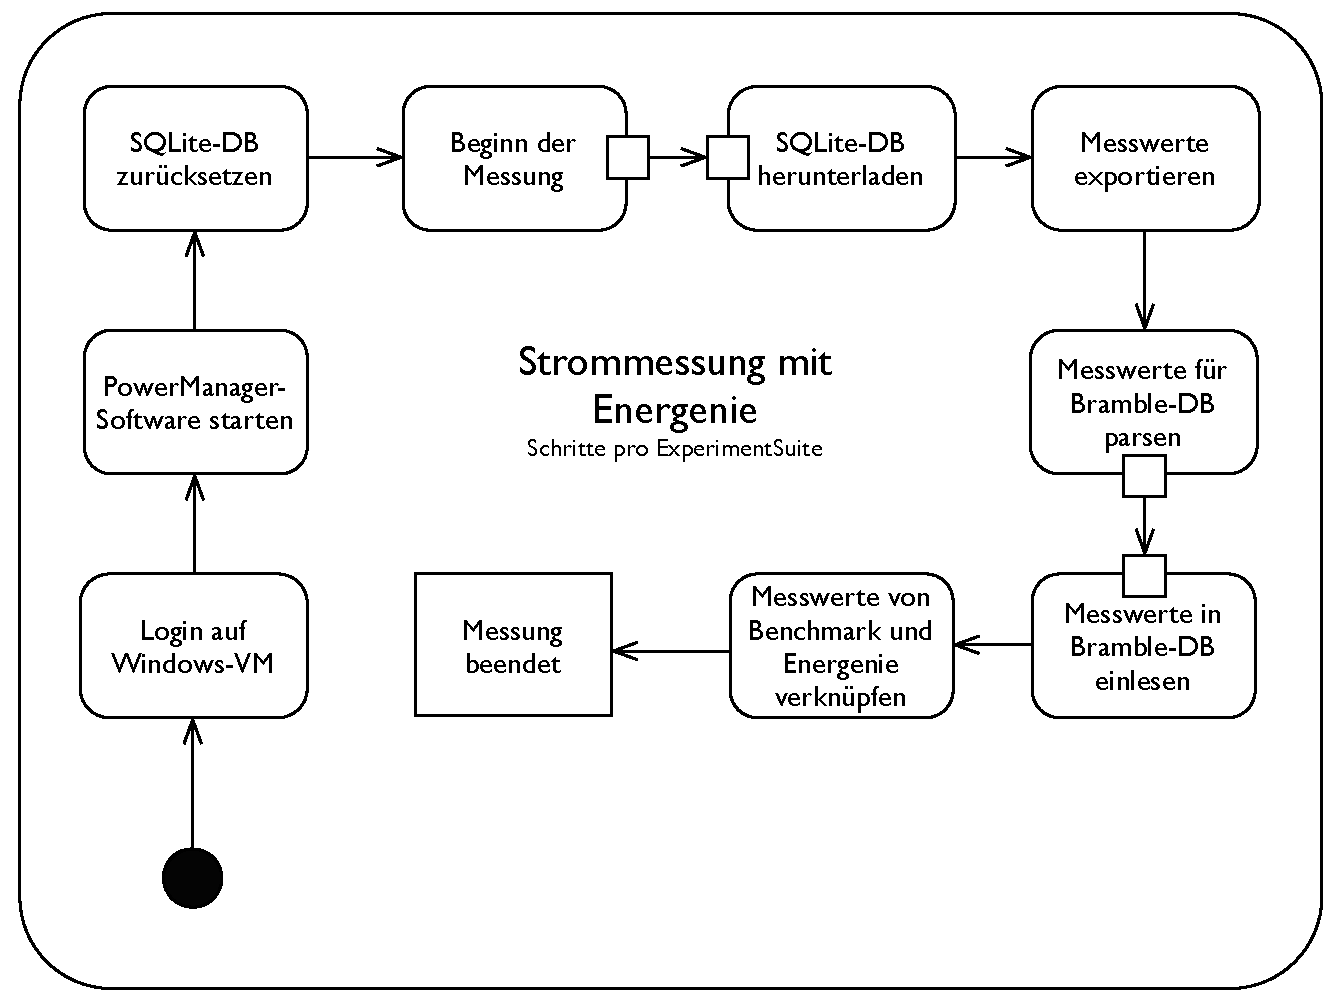
\includegraphics[scale=0.8]{energenie.pdf}\\ 
%  \caption{Aktivit"atsdiagramm zur Durchf"uhrung einer Strommessung f"ur eine ExperimentSuite.}
%  \label{fig:energenie}		
%\end{figure}

\begin{enumerate}\bfseries
% Login auf VM 
	\item Login auf einer Windows-Maschine.
% PowerManager starten 
	\item Starten der PowerManager-Software. 
% Energenie auswählen 
	\item Auswahl des Energenie.
% Datenbank leeren 
	\item Zur"ucksetzen der SQLite-Datenbank.
% Grafische Aufzeichnung starten (optional)
	\item Start der grafischen Aufzeichnung. 
% SQLite-DB herunterladen 
	\item Herunterladen der SQLite-Datenbank. 
% Messwerte parsen für MySQL-DB rpiWerte
	\item Parsen der Messwerte f"ur die Bramble-Datenbank. 
% Messwerte von Strommessung und Benchmarks matchen 
	 \item Verkn"upfung der Messwerte von Energenie und Benchmark-Programm. 
\end{enumerate}

\section{Ergebnisse}\label{Ergebnisse}

Der folgende Abschnitt pr"asentiert die Untersuchungsergebnisse f"ur HPLinpack und STREAM auf dem Bramble. Jeder Benchmark wurde zweimal ausgef"uhrt. Bei Messreihe 1 waren alle RPi-Knoten angeschaltet, bei Messreihe 2 nur die, auf denen die Benchmark-Programme tats"achlich ausgef"uhrt wurden. \texttt{pi03} als Berechnungsknoten blieb immer angeschaltet und wurde in der Untersuchung nicht ber"ucksichtigt (vgl. Kap. \ref{Versuchsaufbau}).

Da keine Implementierung von Whetstone f"ur eine verteilte Berechnung auf Raspbian existiert, war im Verlauf der Untersuchung vorgegeben worden, Whetstone nicht zu ber"ucksichtigen. HPLinpack in der verwendeten Implementierung ben"otigt mindestens vier CPUs oder parallele Prozesse. Hier wurde jeder CPU, d.h. einem RPi-Knoten, genau ein Prozess zugewiesen, sodass zur Ausf"uhrung von HPLinpack mindestens vier angeschaltete und aktive RPi-Knoten ben"otigt werden. 

Zur besseren Vergleichbarkeit wurde die verteilte Ausf"uhrung von STREAM daran angepasst, d.h. auch STREAM wurde auf mindestens vier RPi-Knoten parallel ausgef"uhrt. 

\subsection{HPLinpack: Performance}\label{Ergebnisse-HPL}

HPLinpack in der verwendeten Implementierung (vgl. Kap. \ref{Linpack-RPi}) liefert folgende Ausgabe:

Zun"achst erfolgt eine Erl"auterung der verwendeten Eingabe- und Ausgabeparameter. Ein Teil der Eingabeparameter ist invariabel (\texttt{eps} bzw. Maschinengenauigkeit und \texttt{T/V} bzw. Ausf"uhrungszeit). Die anderen Eingabeparameter sind in der Datei \texttt{HPL.dat} angegeben, die im selben Verzeichnis wie die ausf"uhrbare Datei des Benchmark-Programms liegen muss. Dazu z"ahlen die Problemgr"o\ss e bzw. Ordnung des zu l"osenden linearen Gleichungssystems \texttt{N}, die Anzahl an verwendeten Problemgr"o\ss en \texttt{\#N}, die Blockgr"o\ss e\texttt{NB}\footnote{Die L"osung des linearen Gleichungssystems erfolgt mittels L/U-Faktorisierung. Dazu wird zun"achst eine $n\times n+1$-Koeffizientenmatrix der Ausgangsmatrix A erzeugt. Diese wird zur weiteren Bearbeitung in Bl"ocke der Gr"o\ss e $NB\times NB$aufgeteilt.} und die Gr"o\ss e des Prozessorennetzes (\texttt{P} und \texttt{Q})\footnote{Die Bl"ocke werden zur Bearbeitung einem Netz aus Prozessoren "ubergeben der Gr"o\ss e $P\times Q$ "ubergeben. \texttt{P} bezeichnet darin die Anzahl von Prozessoren in einer Spalte, \texttt{Q} die Anzahl von Prozessoren in einer Zeile des Netzes.} (vgl. \url{http://www.netlib.org/benchmark/hpl/algorithm.html}). 

Die Ausgabeparameter sind invariabel. Die wichtigsten davon sind \texttt{Gflops} (Ausf"uhrungsrate in GFLOPs) und \texttt{Time} (Ausf"uhrungsdauer in Sekunden). F"ur jede Ausf"uhrung von HPLinpack werden 864 Tests durchgef"uhrt, d.h. 864 Messwerte f"ur Ausf"uhrungsrate und Ausf"uhrungsdauer erzeugt. \texttt{Gflops} wird auf 8, \texttt{Time} auf 2 Nachkommastellen genau angegeben. 

Die Diagramme \ref{fig:hpl1} und \ref{fig:hpl2} zeigen die Ergebnisse von Messreihe 1, jeweils skaliert auf 16--4 RPi-Knoten. Dabei sind jeweils n RPi-Knoten aktiv und alle 20 RPi-Knoten angeschaltet.
\begin{figure}[htb]
  \centering
  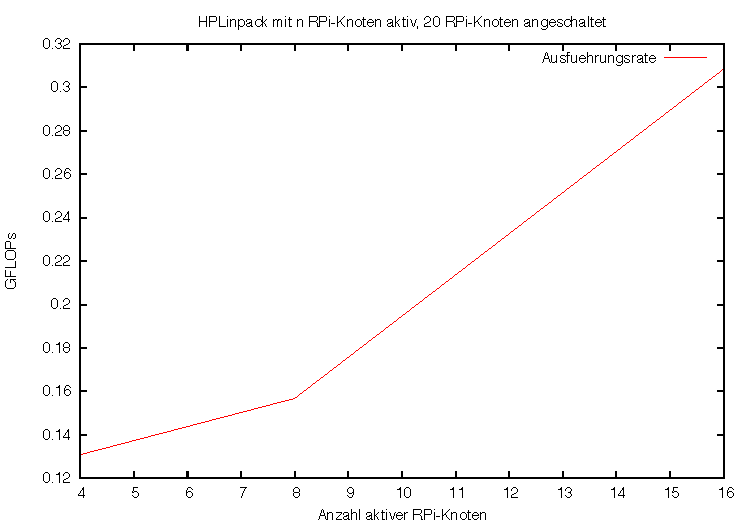
\includegraphics[scale=0.8]{hpl1.pdf}\\ 
  \caption{Ausf"uhrungsrate f"ur HPLinpack, Messreihe 1.}
  \label{fig:hpl1}		
\end{figure}
\begin{figure}[htb]
  \centering
  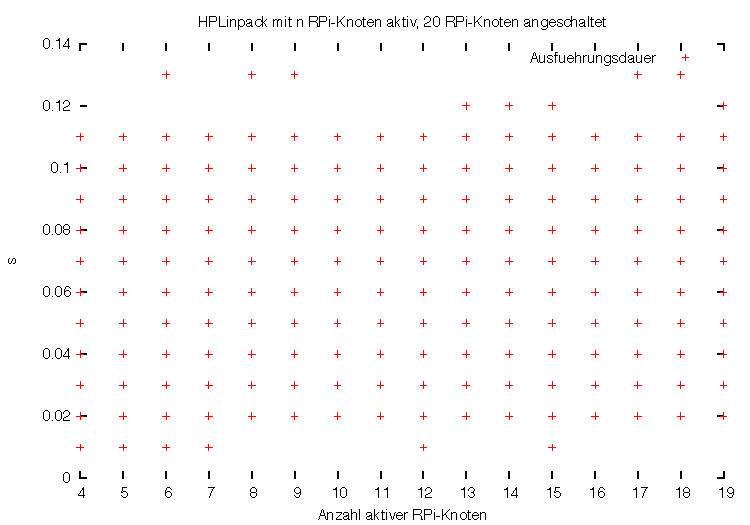
\includegraphics[scale=0.8]{hpl2.pdf}\\ 
  \caption{Ausf"uhrungsdauer f"ur HPLinpack, Messreihe 1.}
  \label{fig:hpl2}		
\end{figure}
\noindent
Die Diagramme \ref{fig:hpl5} und \ref{fig:hpl6} stellen die Ergebnisse von Messreihe 1 denen von Messreihe 2 gegen"uber, in der nicht mehr aktive RPi-Knoten nach der Ausf"uhrung des Benchmarks heruntergefahren werden. Die Ergebnisse von Messreihe 1 sind rot, die von Messreihe 2 blau dargestellt.
\begin{figure}[htb]
  \centering
  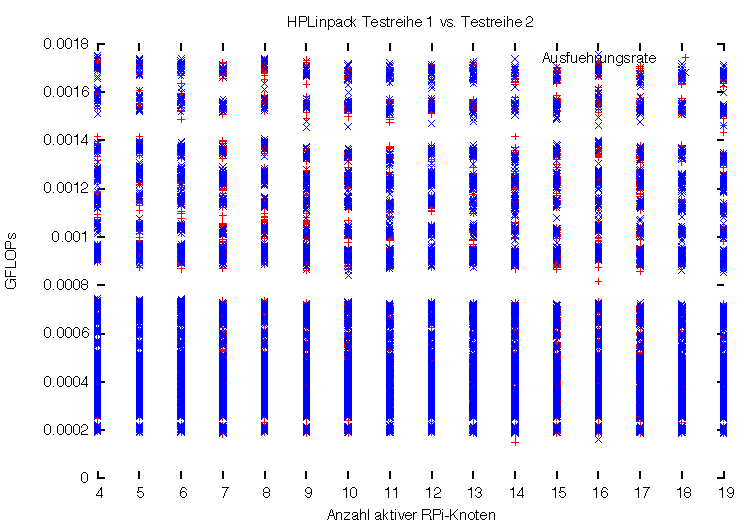
\includegraphics[scale=.8]{hpl5.pdf}\\ 
  \caption{Ausf"uhrungsrate f"ur HPLinpack, Messreihe 1 und Messreihe 2.}\label{fig:hpl5}
\end{figure}
\begin{figure}[htb]
  \centering
  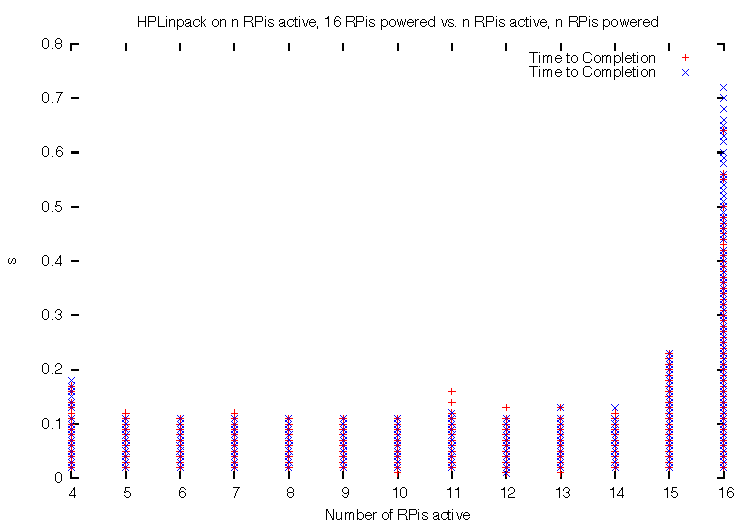
\includegraphics[scale=.8]{hpl6.pdf}\\ 
  \caption{Ausf"uhrungsdauer f"ur HPLinpack, Messreihe 1 und Messreihe 2.}\label{fig:hpl6}
\end{figure}
\subsection{STREAM: Performance}\label{Ergebnisse-Stream}

In der Ausgabe von STREAM werden zun"achst ebenfalls die verwendeten Parameter angegeben, darunter Anzahl an Prozessoren, Vektorl"ange, Speicherbedarf und Anzahl an Iterationen f"ur jedes Modul. F"ur die vier Module Copy, Scale, Add und Triad (vgl. Kap. \ref{Funktion-STREAM}) werden die beste erzielte Ausf"uhrungsrate in MB/s (\texttt{Rate}) und die durchschnittliche (\texttt{Avg time}), minimale (\texttt{Min time}) und maximale Ausf"uhrungsdauer (\texttt{Max time}) in Sekunden ausgegeben. Die Ausf"uhrungsrate wird auf eine, die Ausf"uhrungsdauer auf 6 Nachkommastellen genau angegeben. 

Diagramme \ref{fig:stream1} und \ref{fig:stream2} zeigen die Ergebnisse von Messreihe 1 f"ur STREAM. Ausgabeparameter sind Ausf"uhrungsrate in MB/s und durchschnittliche Ausf"uhrungsdauer in Sekunden f"ur Copy, Scale, Add und Triad, skaliert auf 16--4 RPi-Knoten. Dabei sind jeweils n RPi-Knoten aktiv und alle 20 RPi-Knoten angeschaltet.  
\begin{figure}[htb]
  \centering
  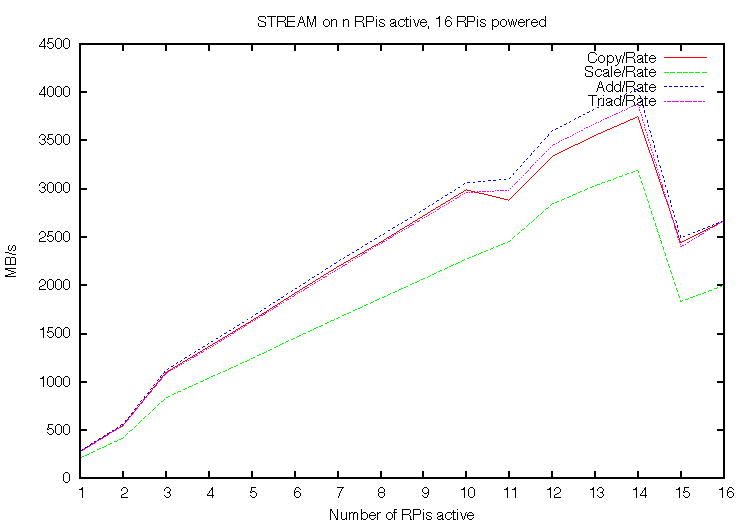
\includegraphics[scale=0.8]{stream1.pdf}\\ 
  \caption{Ausf"uhrungsrate f"ur STREAM, Messreihe 1.}
  \label{fig:stream1}		
\end{figure}
\begin{figure}[htb]
  \centering
  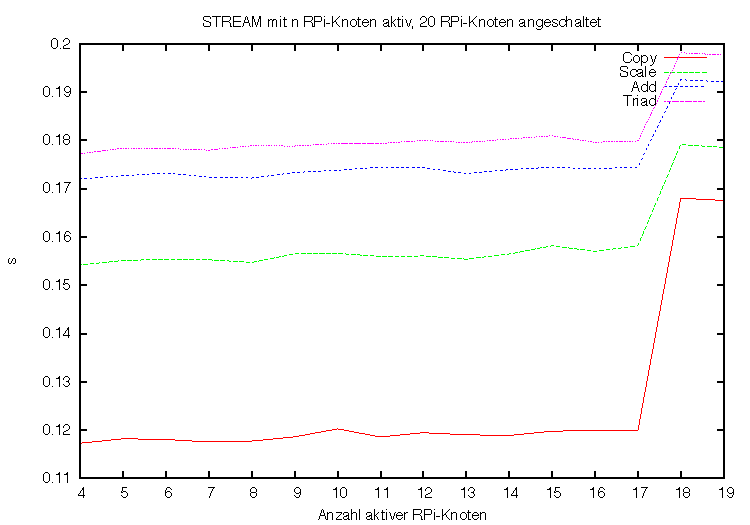
\includegraphics[scale=0.8]{stream2.pdf}\\ 
  \caption{Ausf"uhrungsdauer f"ur STREAM, Messreihe 1.}
  \label{fig:stream2}		
\end{figure}
\noindent
Die Diagramme \ref{fig:stream5} und\ref{fig:stream6} stellen die Ergebnisse von Messreihe 1 und Messreihe 2 f"ur STREAM gegen"uber. Auch hier sind die Ergebnisse von Messreihe 1 rot, die von Messreihe 2 blau markiert. 
\begin{figure}[htb]
  \centering
  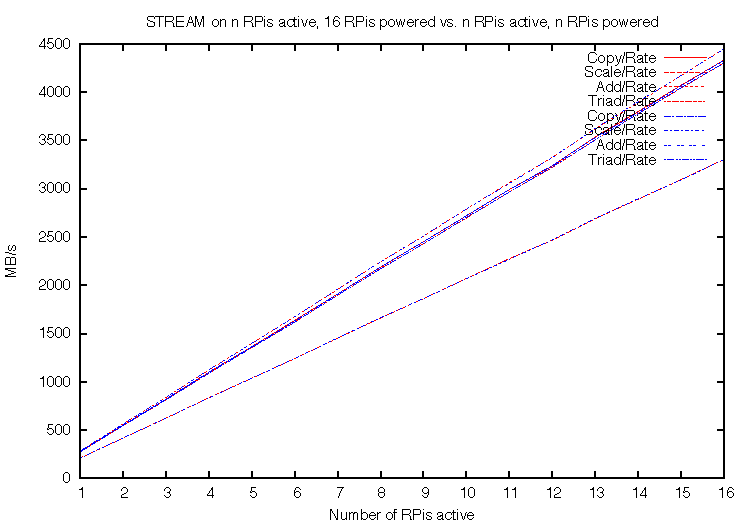
\includegraphics[scale=.8]{stream5.pdf}\\ 
  \caption{Ausf"uhrungsrate f"ur STREAM, Messreihe 1 und Messreihe 2.}\label{fig:stream5}
\end{figure}
\begin{figure}[htb]
  \centering
  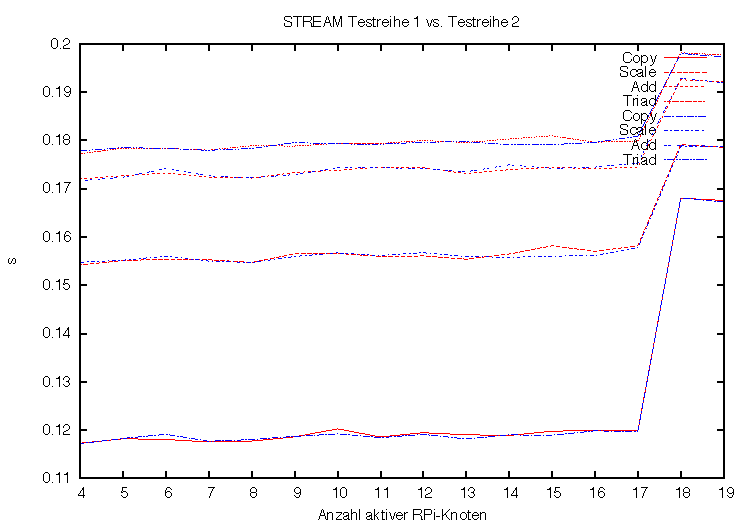
\includegraphics[scale=.8]{stream6.pdf}\\ 
  \caption{Ausf"uhrungsdauer f"ur STREAM, Messreihe 1 und Messreihe 2.}\label{fig:stream6}
\end{figure}
\subsection{Stromverbrauch}\label{Ergebnisse-Energenie}

Die Diagramme \ref{fig:strom1} und \ref{fig:strom2} zeigen die Ergebnisse der Strommessung f"ur die Messreihen 1 und 2. Diagramm \ref{fig:strom1} zeigt den Energieverbrauch in Watt, wenn alle 20 RPi-Knoten angeschaltet sind. Diagramm \ref{fig:strom2} zeigt den Energieverbrauch, wenn nicht mehr aktive RPi-Knoten heruntergefahren werden. 
%TODO: 
%\begin{figure}[htb]
%  \centering
%  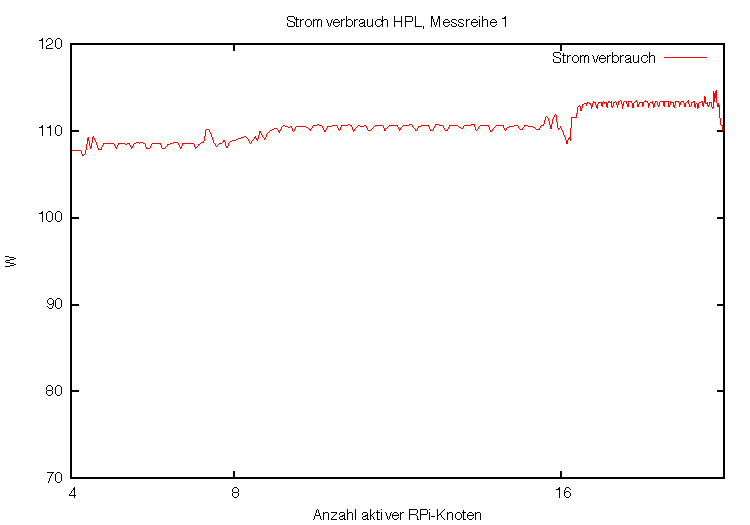
\includegraphics[scale=.8]{strom1.pdf}\\ 
%  \caption{Energieverbrauch in W f"ur HPLinpack mit n RPi-Knoten aktiv/20 RPi-Knoten angeschaltet.}\label{fig:strom1}
%\end{figure}
%\begin{figure}[htb]
%  \centering
%  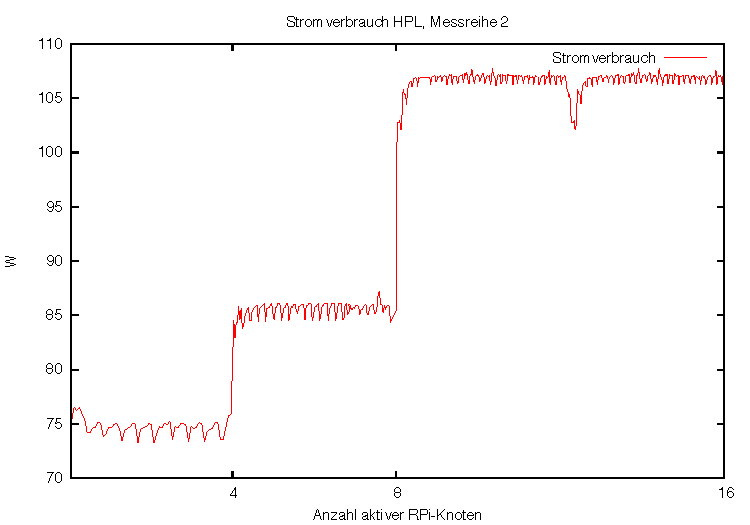
\includegraphics[scale=.8]{strom2.pdf}\\ 
%  \caption{Energieverbrauch in W f"ur STREAM mit n RPi-Knoten aktiv/n RPi-Knoten angeschaltet.}\label{fig:strom2}
%\end{figure}
\endinput 



	\chapter{Interpretation}\label{Kap4}

Das folgende Kapitel dient der Bewertung und Einordnung der Untersuchungsergebnisse. Im Fokus steht dabei das Skalierungsverhalten des Bramble.    

\section{HPL: Performance}\label{Interpretation-Linpack}
Wie in Kapitel \ref{Ergebnisse-HPL} dargestellt, besteht ein proportionales Verh"altnis zwischen dem Quadrat der Problemgr"o\ss e und der Gr"o\ss e des Gesamthauptspeichers. Somit ist bei Hinzunahme von Ressourcen in Form von RPi-Knoten ein linearer Anstieg der Ausf"uhrungsrate zu erwarten. Das gilt ebenfalls f"ur die Ausf"uhrungsdauer. Abbildungen \ref{fig:hpl1} und \ref{fig:hpl2} best"atigen die Erwartungen: Der Anstieg der Ausf"uhrungsdauer ist nahezu linear und betr"agt im Mittel 0.031 GFLOPs pro zus"atzlicher Ressource. Die maximale Abweichung hiervon betr"agt 0.008 GFLOPs. Der Anstieg der Ausf"uhrungdauer ist nahezu linear und betr"agt im Mittel 13.28 s. Die maximale Abweichung hiervon betr"agt 8.24 s.

Das Skalierungsverhalten des Bramble bei der Ausf"uhrung von HPL kann somit als erwartungsgem"a\ss\ bezeichnet werden.

Versuchsaufbau und Funktionsweise des Benchmarks lassen erwarten, dass sich kein signifikanter Unterschied in Ausf"uhrungsrate und Ausf"uhrungsdauer zeigt, wenn nicht an der Programmausf"uhrung beteiligte RPi-Knoten heruntergefahren werden. Abbildungen \ref{fig:hpl5} und \ref{fig:hpl6} best"atigen diese Erwartung: Messreihe 1 und Messreihe 2 werden nahezu identisch dargestellt. Die Ausf"uhrungsdauer in Messreihe 2 ist geringf"ugig h"oher als in Messreihe 1. Die Abweichung betr"agt im Mittel 0.41 s. Die maximale Abweichung betr"agt 0.63 s. Die Ausf"uhrungsrate ist in Messreihe 2 f"ur $n=4$ und $n=16$ RPi-Knoten geringf"ugig niedriger als in Messreihe 1. Die Abweichung betr"agt im Mittel 0.001 GFLOPs (gerundet auf drei Nachkommastellen an Hand der Messgenauigkeit, vgl. Kap. \ref{Ergebnisse-HPL}). Die maximale Abweichung betr"agt 0.001 GFLOPs. 

Es l"asst sich schlussfolgern, dass das Herunterfahren nicht mehr aktiver RPi-Knoten keine signifikanten Auswirkungen auf Ausf"uhrungsrate und Ausf"uhrungsdauer von HPL auf dem Bramble hat. Das Skalierungsverhalten in Messreihe 1 und Messreihe 2 kann als gleich bezeichnet werden. 
%\newpage
\section{STREAM: Performance}\label{Interpretation-Stream}

Die Funktionsweise des Benchmarks l"asst einen linearen Anstieg der Ausf"uhrungsrate bei der Hinzunahme von Ressourcen erwarten. F"ur die Ausf"uhrungsdauer auf jeder einzelnen CPU ist ein konstantes Verhalten zu erwarten. Abbildungen \ref{fig:stream1} und \ref{fig:stream2} best"atigen die Erwartungen f"ur $n\leq 17$ RPi-Knoten: Der Anstieg der Ausf"uhrungsdauer ist nahezu linear und betr"agt im Mittel 245.9 MB/s (Copy), 205.1 MB/s (Scale), 275.5 MB/s (Add) bzw. 266.9 MB/s (Triad) pro zus"atzlicher Ressource. Die maximale Abweichung hiervon betr"agt 54.2 MB/s (Copy), 19.7 MB/s (Scale), 25.9 MB/s (Add) bzw. 25.6 MB/s (Triad). Die Ausf"uhrungsdauer verh"alt sich nahezu konstant und betr"agt im Mittel 0.118791 s (Copy), 0.156077 (Scale), 0.173474 (Add) bzw. 0.179196 (Triad). Die maximale Abweichung hiervon betr"agt 0.001525 s (Copy), 0.002114 s (Scale), 0.002463 s (Add) bzw. 0.003793 s (Triad). 

Das Skalierungsverhalten des Bramble bei der Ausf"uhrung von STREAM kann somit f"ur $n\leq 17$ RPi-Knoten als erwartungsgem"a\ss\ bezeichnet werden. 

Versuchsaufbau und Funktionsweise des Benchmarks legen nahe, dass sich kein signifikanter Unterschied in Ausf"uhrungsrate und Ausf"uhrungsdauer zeigt, wenn nicht an der Programmausf"uhrung beteiligte RPi-Knoten heruntergefahren werden. Abbildungen \ref{fig:stream5} und \ref{fig:stream6} best"atigen diese Erwartung f"ur $n\leq 17$ RPi-Knoten: Ausf"uhrungsraten von Messreihe 1 und Messreihe 2 werden nahezu identisch dargestellt. Die Abweichung von Messreihe 2 gegen"uber Messreihe 1 betr"agt im Mittel 0.1 MB/s (Copy), 0.5 MB/s (Scale), 2.9 MB/s (Add) bzw. 2.95 MB/s (Triad). Die maximale Abweichung gegen"uber Messreihe 1 betr"agt 25.4 MB/s (Scale auf $n=16$ RPi-Knoten). Bei der Ausf"uhrungsdauer betr"agt die Abweichung gegen"uber Messreihe 1 im Mittel 0.000123 s (Copy), 0.000129 s (Scale), 0.000190 s (Add) bzw. 0.000122 s (Triad). Die maximale Abweichung gegen"uber Messreihe 1 betr"agt 0.000823 s (Copy auf $n=15$ RPi-Knoten). 

F"ur $n\leq 17$ RPi-Knoten l"asst sich schlussfolgern, dass das Herunterfahren nicht mehr aktiver RPi-Knoten keine signifikanten Auswirkungen auf Ausf"uhrungsrate und Ausf"uhrungsdauer von STREAM auf dem Bramble hat. Das Skalierungsverhalten in Messreihe 1 und Messreihe 2 kann f"ur $n\leq 17$ RPi-Knoten als gleich bezeichnet werden.

F"ur $n > 17$ RPi-Knoten weicht das Skalierungsverhalten des Bramble von den Erwartungen ab. Abbildung \ref{fig:stream-abweichung} stellt erwartete und erzielte Messwerte f"ur Messreihe 1 gegen"uber. Abweichungen von mehr als 1 MB/s (Ausf"uhrungsrate) und 0.01 s (Ausf"uhrungsdauer) gegen"uber den erwarteten Werten sind rot markiert. Die erwarteten Werte werden f"ur \textit{n} RPi-Knoten wie folgt bestimmt: 
\[\text{Erwartete Performance} = \frac{\text{Performance f"ur }n=17}{17}\ast n\] 
\[\text{Erwartete Ausf"uhrungsdauer = Durchschnittliche Ausf"uhrungsdauer f"ur }n\leq 17\]
\begin{figure}[htb]
  \centering
  \begin{tabular}{|l|c|c|c|}
    \hline 
    \textbf{Aktive RPis:} & \textbf{17} & \textbf{18} & \textbf{19}\\ 
    \hline 
    \textbf{Copy in MB/s (erwartet):} & 4556.4 & 4824.4 & 5092.5\\
    \hline 
    \textbf{Copy in MB/s (erzielt):} & 4556.4 & \textcolor{red}{3451.6} & \textcolor{red}{3642.9}\\
    \hline 
    \textbf{Copy in s (erwartet):} & 0.118791 & 0.118791 & 0.118791\\
    \hline 
    \textbf{Copy in s (erzielt):} & 0.119821 & \textcolor{red}{0.168030} & \textcolor{red}{0.167579}\\
    \hline 
    \textbf{Scale in MB/s (erwartet):} & 3497.7 & 3703.5 & 3909.1\\
    \hline 
    \textbf{Scale in MB/s (erzielt):} & 3497.7 & \textcolor{red}{3236.2} & \textcolor{red}{3421.8}\\
    \hline 
	\textbf{Scale in s (erwartet):} & 0.156077 & 0.156077 & 0.156077\\
    \hline 
    \textbf{Scale in s (erzielt):} & 0.158162 & \textcolor{red}{0.179140} & \textcolor{red}{0.178560}\\
    \hline 
    \textbf{Add in MB/s (erwartet):} & 1672.5 & 4978.6 & 5255.2\\
    \hline 
    \textbf{Add in MB/s (erzielt):} & 1672.5 & \textcolor{red}{4501.4} & \textcolor{red}{4765.8}\\
    \hline 
    \textbf{Add in s (erwartet):} & 0.173474 & 0.173474 & 0.173474\\
    \hline 
    \textbf{Add in s (erzielt):} & 0.174494 & \textcolor{red}{0.192586} & \textcolor{red}{0.192147}\\
    \hline 
    \textbf{Triad in MB/s (erwartet):} & 4557.4 & 4852.5 & 4093.6\\
    \hline 
    \textbf{Triad in MB/s (erzielt):} & 4557.4 & \textcolor{red}{4377.4} & \textcolor{red}{4632.1}\\
    \hline 
    \textbf{Triad in s (erwartet):} & 0.179196 & 0.179196 & 0.179196\\
    \hline 
    \textbf{Triad in s (erzielt):} & 0.179882 & \textcolor{red}{0.198159} & \textcolor{red}{0.197686}\\
    \hline 
  \end{tabular}
  \caption{Erwartete und erzielte Messwerte f"ur STREAM auf $n\geq 17$ RPi-Knoten.}\label{fig:stream-abweichung}
\end{figure}
\newpage
\noindent
Es stellt sich die Frage, warum f"ur $n>17$ RPi-Knoten eine deutlich schlechtere Performance und verl"angerte Ausf"uhrungsdauer auftreten. Folgende Erkl"arungen sind denkbar: 
\begin{enumerate}\bfseries
	\item Funktionsweise des Benchmarks.\\
\normalfont
Wie zu Beginn des Kapitels dargestellt, ist bei der Hinzunahme von Ressourcen auf einem Rechencluster mit einem linearen Anstieg der Ausf"uhrungszeit und ann"ahernd konstanter Ausf"uhrungsdauer zu rechnen. McCalpin schreibt hierzu: 
\begin{quote}
\onehalfspacing
[\dots] unless something is very wrong, the performance of a cluster will be the performance of a node times the number of nodes (vgl. \url{http://www.cs.virginia.edu/stream/ref.html}).
\end{quote} 
Ein erw"unschter Effekt ist somit nach der Funktionsweise des Benchmarks auszuschlie\ss en. 
	\textbf{\item Architektur des Bramble.}\\
M"ogliche Ursachen sind Systemzeit, Netzwerk und Netz-Dateisystem. 

Wie in Kap. \ref{Bramble-Versuchsaufbau} dargestellt, hat der RPi keine eingebaute Systemuhr. Die Zeitsynchronisation der RPi-Knoten erfolgt einmal beim Bootvorgang gegen"uber dem Open\-NTP-Server auf \texttt{careme} (vgl. \cite{kli13}). Wenn Rechenlast ungleich auf die RPi-Knoten verteilt wird und die beteiligten CPUs sehr ausgelastet sind, w"are es denkbar, dass die Systemzeit dieser Knoten driftet und zu abweichenden Messergebnissen bei der Ausf"uhrungsdauer f"uhrt. Dieser Effekt kann hier ausgeschlossen werden: Die Rechenlast ist bei $n\leq 17$ Knoten nicht weniger ungleich verteilt ist als bei $n>17$ Knoten, sodass der Effekt schon fr"uher eintreten m"usste. Die Rechenlast der parallelen Ausf"uhrung von STREAM ist zudem f"ur alle beteiligten Knoten gleich. 

Wie in Kap. \ref{Bramble-Spezi} dargestellt, sind Server und RPi-Knoten "uber ein Ethernet-Netzwerk verbunden. Wie bei \cite{kli13} erl"autert, kann damit ein maximaler Datendurchsatz von ca. 2 MB/s erreicht werden. Ein Erkl"arungsansatz war das "Uberschreiten dieser Obergrenze bei mehr als 17 parallelen Ausf"uhrungen. 

Bez"uglich der Bandbreiten zeigte sich durch Nachrechnen eine Steigerung um rund 35 MB  f"ur Copy und Scale pro zus"atzlichem RPi-Knoten. F"ur Add und Triad erfolgt eine Steigerung um rund 50 MB. Hierbei handelt es sich nat"urlich nicht um den Durchsatz des Netzwerks, sondern um den Durchsatz von Hauptspeicherzugriffen jedes einzelnen RPi-Knotens. Diese Steigerung erfolgt auch bei $n>17$
RPi-Knoten. Der Durchsatz von Hauptspeicherzugriffen verh"alt sich somit erwartungsgem"a\ss\ f"ur alle \textit{n}. Ein "Uberschreiten des maximalen Netzwerk-Datendurchsatzes scheidet somit als Ursache aus. 

Binaries und verwendete Bibliotheken der Benchmarks liegen im geteilten Verzeichnis \texttt{/srv}. Es erschien denkbar, dass mehr als 17 parallele Zugriffe darauf das Netz-Dateisystem "uberlasten. Deswegen wurde probeweise auf den SD-Karten aller RPi-Knoten eine neue Partition erstellt und der Inhalt des geteilten Verzeichnisses hinein kopiert. In der Datei \texttt{/etc/fstab} aller RPi-Knoten wurde der Mountpoint f"ur \texttt{/srv} tempor"ar entsprechend ge"andert. Das Resultat waren Performance-Einbr"uche bei STREAM schon ab $n=13$ RPi-Knoten, womit das Netz-Dateisystem als Ursache ausscheidet.
\textbf{\item Ausf"uhrung des Benchmarks.}\\
Eine m"ogliche Ursache ist die Funktionsweise von MPICH.

Wie in Kap. \ref{Versuchsaufbau} und \ref{Bramble-Versuchsaufbau} beschrieben, wird die parallele Ausf"uhrung von STREAM durch MPICH angesto\ss en, das den im Machinefile spezifizierten CPUs eine bestimmte Anzahl an parallelen Programmaufrufen zuweist. Ein weiterer Erkl"arungsansatz war die "Uberlastung des Netzwerks durch den Kommunikations-Overhead ab einem Schwellenwert von $n=18$ parallelen Programmaufrufen. 

MPI nutzt zur Interprozesskommunikation u.a. Broadcast- und Unicast-Nachrichten. Bei der parallelen Ausf"uhrung von Anwendungen werden meist die Funktionen \texttt{MPI\_\-Bcast} und \texttt{MPI\_Gather} aufgerufen. Hierbei schickt ein Root-Prozess entweder eine Nachricht an alle beteiligten CPUs bzw. Prozesse oder sammelt die Daten aller beteiligten CPUs bzw. Prozesse ein (vgl. \cite{pie12}). Es erschien denkbar, dass eine Broadcast-Nachricht an mehr als 17 Prozessoren das Netzwerk "uberlastet und zu den beobachteten Performance-Einbr"uchen f"uhrt. Daher wurde der Quellcode von STREAM testweise so ver"andert, dass jedes Modul 100 Mal statt zehn Mal ausgef"uhrt wird\footnote{Dazu muss die Variable \texttt{ntimes} ver"andert werden, vgl. \url{http://www.cs.virginia.edu/stream/ref.html}.}. Bei einer l"angeren Ausf"uhrungsdauer des Programms war zu erwarten, dass der Kommunikations-Overhead von MPICH abnimmt und erwartungsgem"a\ss e Performance-Resultate erzielt werden. Das war nicht der Fall. Abbildung \ref{fig:stream-ntimes100} stellt dar, welche Ergebnisse f"ur $n=18$ RPi-Knoten erzielt wurden. 
\begin{figure}[H]
  \centering
  \begin{tabular}{|l|c|}
    \hline 
    \textbf{Aktive RPi-Knoten:} & \textbf{18}\\ 
    \hline 
    \textbf{Copy in MB/s (erwartet):} & 4824.4\\
    \hline 
    \textbf{Copy in MB/s (erzielt):} & \textcolor{red}{3398.3}\\
    \hline 
    \textbf{Copy in s (erwartet):} & 0.118791\\
    \hline 
    \textbf{Copy in s (erzielt):} & \textcolor{red}{0.170848}\\
    \hline 
    \textbf{Scale in MB/s (erwartet):} & 3703.5\\
    \hline 
    \textbf{Scale in MB/s (erzielt):} & \textcolor{red}{3189.5}\\
    \hline 
	\textbf{Scale in s (erwartet):} & 0.156077\\
    \hline 
    \textbf{Scale in s (erzielt):} & \textcolor{red}{0.181711}\\
    \hline 
    \textbf{Add in MB/s (erwartet):} & 4978.6\\
    \hline 
    \textbf{Add in MB/s (erzielt):}& \textcolor{red}{4373.3}\\
    \hline 
    \textbf{Add in s (erwartet):} & 0.173474\\
    \hline 
    \textbf{Add in s (erzielt):} & \textcolor{red}{0.199341}\\
    \hline 
    \textbf{Triad in MB/s (erwartet):} & 4852.5\\
    \hline 
    \textbf{Triad in MB/s (erzielt):} & \textcolor{red}{4149.8}\\
    \hline 
    \textbf{Triad in s (erwartet):} & 0.179196\\
    \hline 
    \textbf{Triad in s (erzielt):} & \textcolor{red}{0.209507}\\
    \hline 
  \end{tabular}
  \caption{Erwartete und erzielte Messwerte f"ur STREAM auf $n=18$ RPi-Knoten mit \texttt{ntimes=100}.}\label{fig:stream-ntimes100}
\end{figure}
\noindent
Die Resultate fallen noch schlechter aus als bei STREAM auf $n=18$ RPi-Knoten mit \texttt{ntimes=10} (vgl. Abbildung \ref{fig:stream-abweichung}). Damit scheidet ein Kommunikations-Overhead von MPICH als Erkl"arung aus. Die Ursache konnte somit nicht zweifelsfrei gekl"art werden. 
\end{enumerate}

\section{Stromverbrauch}
Ziel der Strommessung war die Ermittlung des Skalierungsverhaltens des Bramble bez"uglich des Stromverbrauchs. In Messreihe 1 werden laufend Ressourcen in Form von RPi-Knoten hinzugenommen. Auch nicht aktive RPi-Knoten sind angeschaltet, nehmen somit Strom auf. In Messreihe 2 werden nicht aktive RPi-Knoten abgeschaltet, nehmen somit keinen Strom auf. 

Es ist zu erwarten, dass der Stromverbrauch deutlich sinkt, wenn nicht aktive RPi-Knoten von der Stromversorgung getrennt werden. Zur "Uberpr"ufung dieser Erwartung wurden Stromverbrauch bei der Ausf"uhrung von HPL und STREAM (Messreihe 1 und Messreihe 2), Zuwachs pro aktivem RPi-Knoten (Messreihe 1) und Zuwachs pro angeschaltetem und aktivem RPi-Knoten (Messreihe 2) empirisch ermittelt. 

Die Ergebnisse werden in Abbildung \ref{fig:stromvergleich} als Mittelwerte dargestellt (gerundet auf 4 Stellen ohne f"uhrende Nullen an Hand der Messgenauigkeit, vgl. Kap. \ref{Strommessung}). 
\begin{figure}[H]
  \centering
  \begin{tabular}{|l|c|c|c|c|}
    \hline 
    & HPL (1) & HPL (2) & STREAM (1) & STREAM (2)\\ 
    \hline 
	\textbf{ExperimentSuite} & 110 W & 88 & 111 W & 94 W\\
    \hline 
    \textbf{Maximale Abweichung} & 4 W & 3 W & 5 W & 5 W\\
	\hline
    \textbf{Zuwachs pro RPi-Knoten} & 0 W & 8 W & 0 W & 2 W\\
    \hline 
    \textbf{Messreihe} & 111 W & 88 W & 111 W & 94 W\\
    \hline 
  \end{tabular}
  \caption{Stromverbrauch des Bramble, Messreihe 1 und Messreihe 2.}
\label{fig:stromvergleich}
\end{figure}
\noindent
Die Messergebnisse best"atigen die Erwartung, dass der Stromverbrauch des Bramble pro abgeschaltetem RPi-Knoten deutlich abnimmt: Im Mittel um 8 W pro RPi-Knoten bei der Ausf"uhrung von HPL und um 2 W pro RPi-Knoten bei der Ausf"uhrung von STREAM. Die Stromverbrauch bei der Durchf"uhrung von Messreihe 2 ist damit im Mittel um 23 W (HPL) bzw. 17 W (STREAM) niedriger als in Messreihe 1. Das Skalierungsverhalten des Bramble bez"uglich des Stromverbrauchs kann somit als erwartungsgem"a\ss\ bezeichnet werden. 
\endinput 
%	\chapter{Zusammenfassung und Ausblick}\label{Kap5}
\begin{quote}
\onehalfspacing
I have converted my Classic Benchmarks to run on the Linux based Raspberry Pi. These are Whetstone, [...], Linpack and Livermore Loops. [...] The Livermore Loops benchmark was used to accept the first supercomputer. So the main bragging rights are:

In 1978, the Cray 1 supercomputer cost \$7 Million, weighed 10,500 pounds and had a 115 kilowatt power supply. It was, by far, the fastest computer in the world. The Raspberry Pi costs around \$70 (CPU board, case, power supply, SD card), weighs a few ounces, uses a 5 watt power supply and is more than 4.5 times faster than the Cray 1. 

My bragging rights are that I developed and ran benchmarks, including Whetstones, on Serial 1 Cray 1\footnote{Quelle: \url{http://www.raspberrypi.org/forum/viewtopic.php?f=31&t=44080}.}.
\end{quote}

In der vorliegenden Arbeit wurde versucht, HPC-Benchmarks auf einem RPi-Cluster lauff"ahig zu machen und zu evaluieren. Dieser Proof of Concept war erfolgreich: 

Die ausgew"ahlten HPC-Benchmarks konnten mit Ausnahme von Whetstone nach dem Ausschluss vorhandener St"orfaktoren auf dem Bramble ausgef"uhrt werden. Die ExperimentSuite konnte mit kleinen "Anderungen am bestehenden Datenbank-Schema in den "ubergeordneten Versuchsaufbau integeriert werden. Die erzielten Messwerte ergaben ein koh"arentes Bild, wurden denen eines RPi-Einzelrechners gegen"ubergestellt sowie in den gr"o\ss eren Kontext der Top500-Rankings und der bisher erzielten Messwerte der Benchmark-Autoren eingeordnet. 

Der Versuchsaufbau reiht sich damit Bestrebungen der letzten Monate, einen Beowulf-Cluster aus Raspberry Pi-Einzelrechnern f"ur verteilte Berechnungen heranzuziehen. Wie Longbottom im obigen Zitat und die Projektleiter der Bramble-Projekte schreiben: Der Raspberry Pi ist in die Welt der Cluster und (zumindest ehemaligen) Supercomputer eingetreten\footnote{Vgl. auch \url{http://www.cs.virginia.edu/stream/stream_mail/2012/0002.html}.} und erzielt in den betrachteten Kategorien CPU-Performance und Speicher-Band\-breite durchaus respektable Ergebnisse. 

Schwierigkeiten zeigten sich vor allem in der vorhandenen Bramble-Infrastruktur, sowohl Hardware als auch IP/SSH-Kommunikation betreffend. M"ogliche zuk"unftige Arbeiten umfassen daher zwei Felder: 

Der vorhandene Bramble ist deutlich verbesserungsf"ahig. Vor allem die Hardware zeigt Schw"achen, nicht nur die Stromversorgung betreffend. Der physische Aufbau ist extrem beengt, sodass Ziehen und erneutes Einstecken von Mini-USB- und Netzwerkkabeln nur eingeschr"ankt m"oglich ist und die Gefahr besteht, die "ubrige Hardware dabei zu besch"adigen. Da die Unterbrechung der Stromversorgung die einzige M"oglichkeit zum Reboot eines RPi ist und eine unterbrochene Netzwerkverbindung nur durch Triggern des Netzwerkkabels wieder hergestellt werden kann, ist dieser Punkt systemkritisch f"ur zuk"unftige Untersuchungen. Abhilfe lie\ss e sich u.U. durch den Einbau von Reset-Kn"opfen auf den einzelnen RPi-Nodes schaffen\footnote{Vgl. z.B. \url{http://raspi.tv/2012/making-a-reset-switch-for-your-rev-2-raspberry-pi}.}. Auch die Platzierung der RPi-Nodes in einem aufrecht stehenden Rack statt eines liegenden Metallgeh"auses w"are von Vorteil\footnote{Vgl. \cite{kie01} und \cite{cox13}.}, damit die h"aufig ben"otigten Anschl"usse besser zug"anglich sind. 

In einem gr"osseren Rahmen w"are es interessant, fr"uher oder sp"ater auf eine MPI-Implemen\-tierung von Whetstone f"ur Raspbian zur"uckgreifen zu k"onnen. Auch die Evaluierung weiterer, bisher nicht betrachteter HPC-Benchmarks steht noch aus. Die wichtigsten Erkenntnisgewinne sind jedoch zu erwarten, wenn in naher Zukunft hoffentlich ein offener Treiber f"ur die RPi-GPU vorliegt. Nachdem Broadcom vor wenigen Wochen erstmals die vollst"andige Spezifikation der GPU zur Verf"ugung gestellt hat\footnote{Vgl. \url{http://blog.broadcom.com/chip-design/android-for-all-broadcom-gives-developers-keys-\-to-the-videocore-kingdom/}.}, hat die Raspberry Pi Foundation einen entsprechenden Wettbewerb ausgeschrieben\footnote{Vgl. \url{http://www.raspberrypi.org/competition-rules}.}. Die Ergebnisse und neuen Einsatzm"oglichkeiten der bisher kaum anprogrammierbaren GPU, die deutlich leistungsf"ahiger ist als die hier schwerpunktm"a\ss ig untersuchte CPU, d"urfen mit Spannung erwartet werden. 
\endinput

% ---------------------------------------------------------------
\backmatter % ab hier keine Nummerierung mehr
    \listoffigures
    \bibliographystyle{alphadin}
    \bibliography{./Bib/grei14}

\end{document}
